\documentclass[\main.tex]{subfiles}

\chapter{Discussão dos Resultados}

\section{Apresentação e Discussão dos Resultados}
Foram utilizados dois datasets para testar os algoritmos desenvolvidos, de modo a obter
resultados e contextos diferentes. O primeiro \textit{\gls{dataset}} aborda a diferença de
velocidades instantâneas numa estrada, enquanto que o segundo estuda a quantidade
populacional num determinado local.

\subsection{Caso de Estudo das Velocidades Instantâneas}
Este conjunto de dados é de uma rua na cidade de Braga e foi calculada a diferença de
velocidades instantâneas no início e no fim da rua. Podem ser apontadas algumas vantagens
no estudo deste \textit{\gls{dataset}} como: previsão das horas mais sossegadas numa estrada
ou do tráfego diário num determinado local. Na tabela 5.1 está representado um excerto do 
conjunto de dados utilizado para realizar este caso de estudo.\par
\vspace{10pt}
\begin{table}[h!]
\centering
\setlength{\extrarowheight}{5pt}
\setlength{\tabcolsep}{10pt}
\begin{tabular}{|c|c|c|c|}
\hline
\textbf{"timestep"} & \textbf{"temperature"} & \textbf{"precipitation"} & \textbf{"speed\_diff"} \\[5pt]
\hline
2019-04-01 07:00:00 & 12.0 & 0.0 & 11.666666666666668 \\[5pt]
\thinhline
2019-04-01 08:00:00 & 15.0 & 0.0 & 0.0 \\[5pt]
\thinhline
2019-04-01 09:00:00 & 16.0 & 0.0 & 11.0 \\[5pt]
\thinhline
2019-04-01 10:00:00 & 17.0 & 0.0 & 19.333333333333332 \\[5pt]
\thinhline
2019-04-01 11:00:00 & 18.0 & 0.0 & 21.333333333333332 \\[5pt]
\thinhline
2019-04-01 12:00:00 & 18.0 & 0.0 & 17.666666666666668 \\[5pt]
\thinhline
2019-04-01 13:00:00 & 16.0 & 0.0 & 25.0 \\[5pt]
\hline
\end{tabular}
\caption{Excerto do \textit{\gls{dataset}} de velocidades instantâneas}
\end{table}\par

\newpage
Na figura 5.1 pode ser visualizado um diagrama de extremos e quartis do
\textit{\gls{dataset}} de velocidades instantâneas relativo ao mês de abril de 2019.\par
\begin{figure}[h!]
\centering
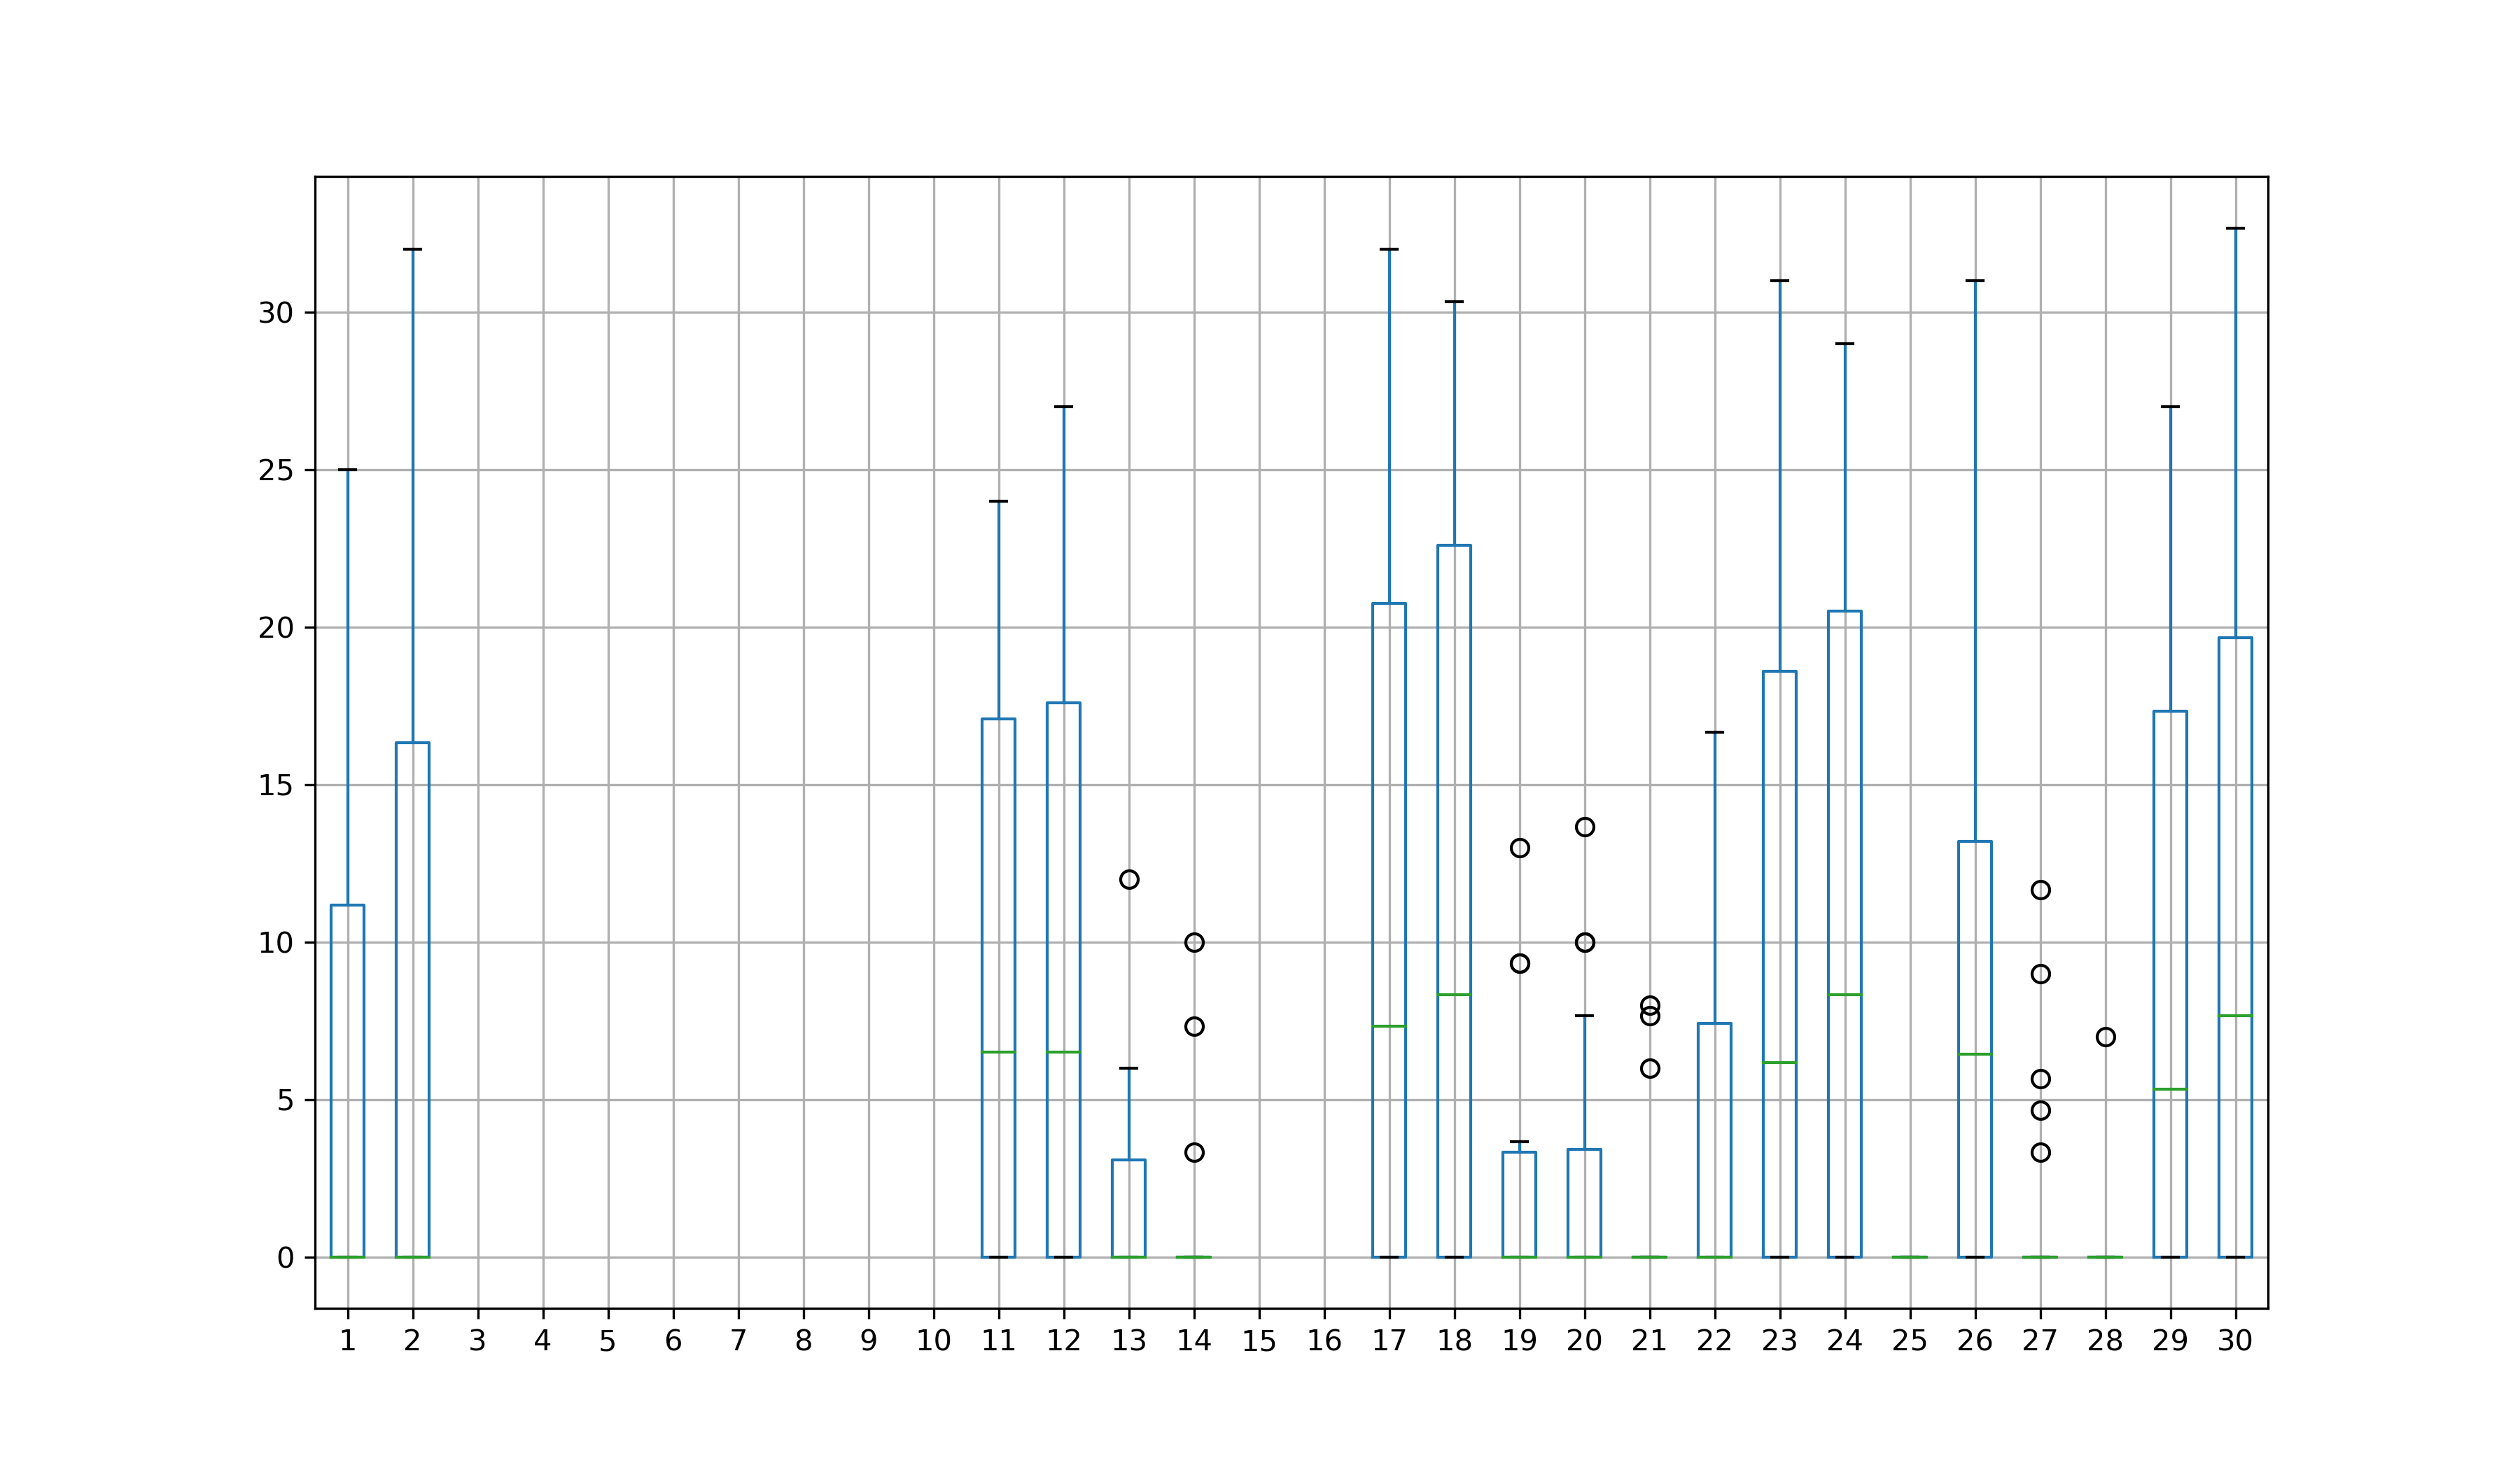
\includegraphics[width=\linewidth]{../private_assets/boxplot_speed_diff_2019_04_dataset.png}
\caption{Diagrama de extremos e quartis do mês de abril de 2019 do \textit{\gls{dataset}} de velocidades instantâneas}
\end{figure}

Algumas perguntas que visam ser respondidas no final deste caso de estudo são:
\begin{itemize}
    \item Qual a melhor hora para andar na estrada de carro?
    \item Qual a pior hora para andar na estrada de carro?
\end{itemize}\par
Para esta série temporal, foram realizadas as \textit{grid searches} da seguinte forma:\par
\begin{enumerate}[label=\roman*)]
    \item Correr \textit{\acrshort{arima}}(p, d, q) com:
    \begin{itemize}
        \item p entre 1 e 5;
        \item d entre 0 e 2;
        \item q entre 0 e 2.
    \end{itemize}
    \item Escolher 4 melhores configurações do \textit{\acrshort{arima}};
    \item Correr \textit{\acrshort{sarima}(p, d, q)(P, D, Q, S)} com as 4 melhores
    configurações dos primeiros parâmetros definidos no passo anterior;
    \item Escolher 2 melhores conjuntos dos parâmetros do \textit{\acrshort{sarima}}.
\end{enumerate}\par
Escolher as variáveis exógenas dos modelos \textit{\acrshort{arimax}} e
\textit{\acrshort{sarimax}} é um pouco mais complexo e exige uma compreensão e estudo do
\textit{\gls{dataset}} em si. Se não for escolhida nenuma variável o modelo não faz sentido
ser executado. Por outro lado, caso seja escolhidas muitas variáveis o modelo ou demora uma
eternidade a terminar ou não retorna resultados nenhuns. Isto significa que, para escolher
estas variáveis é necessário ir testanto as que dão melhores resultados e porquê e,
finalmente, quando estiver a análise feita, juntá-las às configurações iniciais dos
algoritmos.\par
Para terminar, tendo já sido escolhidas as melhores configurações dos dois tipos de
parâmetros, correm-se os modelos todos com as configurações acima descritas. Deste modo, nos
modelos \textit{\acrshort{arima}} e \textit{\acrshort{arimax}} existem 4 possibilidades de
teste e nos modelos \textit{\acrshort{sarima}} e \textit{\acrshort{sarimax}} existem 8
possibilidades. Isto ajuda imenso na previsão de daodos, porque com a utilização das
pesquisas em grelha, não é necessário correr todas as cofigurações para todos os modelos,
ou seja, demora mesmo muito menos tempo.\par

\begin{table}[h!]
\centering
\setlength{\extrarowheight}{5pt}
\begin{tabular}{|c|c|c|c|}
\hline
\textbf{"Model"} & \textbf{"MAE"} & \textbf{"MSE"} & \textbf{"RMSE"} \\[5pt]
\hline
"ARIMA(1,2,3)\_15\_2" & 0.3863972317002109 & 0.17293853210778598 & 0.41585878866243287 \\[5pt]
\thinhline
"ARIMAX(1,2,3)\_15\_2" & 0.41196228043522987 & 0.19971916779536353 & 0.44689950525298583 \\[5pt]
\thinhline
"ARIMA(4,2,3)\_15\_2" & 0.67084667540561 & 0.5543517148947674 & 0.7445479936812451 \\[5pt]
\thinhline
"ARIMAX(1,2,3)\_15\_1" & 3.367502360913987 & 23.984957736878993 & 4.897444000382137 \\[5pt]
\thinhline
"ARIMA(1,2,3)\_15\_1" & 3.444645163427896 & 25.82468592020841 & 5.0817994765839005 \\[5pt]
\thinhline
"ARIMA(1,2,3)\_15\_3" & 5.482114875372973 & 56.350156969636664 & 7.506674161680169 \\[5pt]
\thinhline
\hline
\end{tabular}
\caption{Excerto sumário de resultados da \textit{\gls{grid search}} do primeiro caso de estudo}
\end{table}\par

A tabela 5.2 representa o sumário de resultados da \textit{\gls{grid search}} do dataset das
velocidades instantâneas.\par
Como pode ser constatado, os 3 primeiros modelos da tabela parecem ser os melhores, pelos erros
mínimos que apresentam. No entanto, a 2ª divisão do \textit{\gls{dataset}} apanhou um conjunto
de resultados todos a zero, ou seja, as previsões não foram complicadas de fazer, porém será
impossível aproveitar os resultados do modelo para qualquer tipo de observação final.\par
Conclui-se assim que os 3 melhores modelos testados para este \textit{\gls{dataset}} foram:\\[10pt]
\indent\textit{\acrshort{arimax}}(1, 2, 3), 1ª divisão do \textit{\gls{dataset}}, com 15 previsões.
Representado na tabela 5.3 e na figura 5.2;\\
\indent\textit{\acrshort{arima}}(1, 2, 3), 1ª divisão do \textit{\gls{dataset}}, com 15 previsões.
Representado na tabela 5.4 e na figura 5.3;\\
\indent\textit{\acrshort{arima}}(1, 2, 3), 3ª divisão do \textit{\gls{dataset}}, com 15 previsões.
Representado na tabela 5.5 e na figura 5.4;\\[10pt]

\newpage

\begin{figure}[h!]
\begin{floatrow}
\capbtabbox{%
  \setlength{\extrarowheight}{1pt}
  \begin{tabular}{|c|c|} \hline
    \textbf{"Predict"} & \textbf{"speed\_diff"} \\[1pt] \hline
    0.13817744331334328 & 0.0 \\[1pt] \thinhline
    -0.8973439961623095 & 7.66666666666 6 668 \\[1pt] \thinhline
    7.323374989923932 & 13.66666666666 6 664 \\[1pt] \thinhline
    11.038172786531765 & 0.0 \\[1pt] \thinhline
    2.103461054155741 & 3.0 \\[1pt] \thinhline
    2.091510219928224 & 3.0 \\[1pt] \thinhline
    3.208279408032984 & 3.33333333333 3 333 \\[1pt] \thinhline
    2.283585816926894 & 3.666666666666 6 665 \\[1pt] \thinhline
    3.9253583100976295 & 1 0.0 \\[1pt] \thinhline
    8.34553662378711 & 0.0 \\[1pt] \thinhline
    1.5898776295568244 & 4.0 \\[1pt] \thinhline
    2.7362308186284343 & 0.0 \\[1pt] \thinhline
    0.3293245341001239 & 0.0 \\[1pt] \thinhline
    -0.8090669648652083 & 0.0 \\[1pt] \thinhline
    0.4107963416104033 & 0.0 \\[1pt] \hline
  \end{tabular}
}{%
  \caption{Previsões do modelo \textit{\acrshort{arimax}}(1, 2, 3), 1ª divisão do dataset, com 15 previsões}%
}
\ffigbox{%
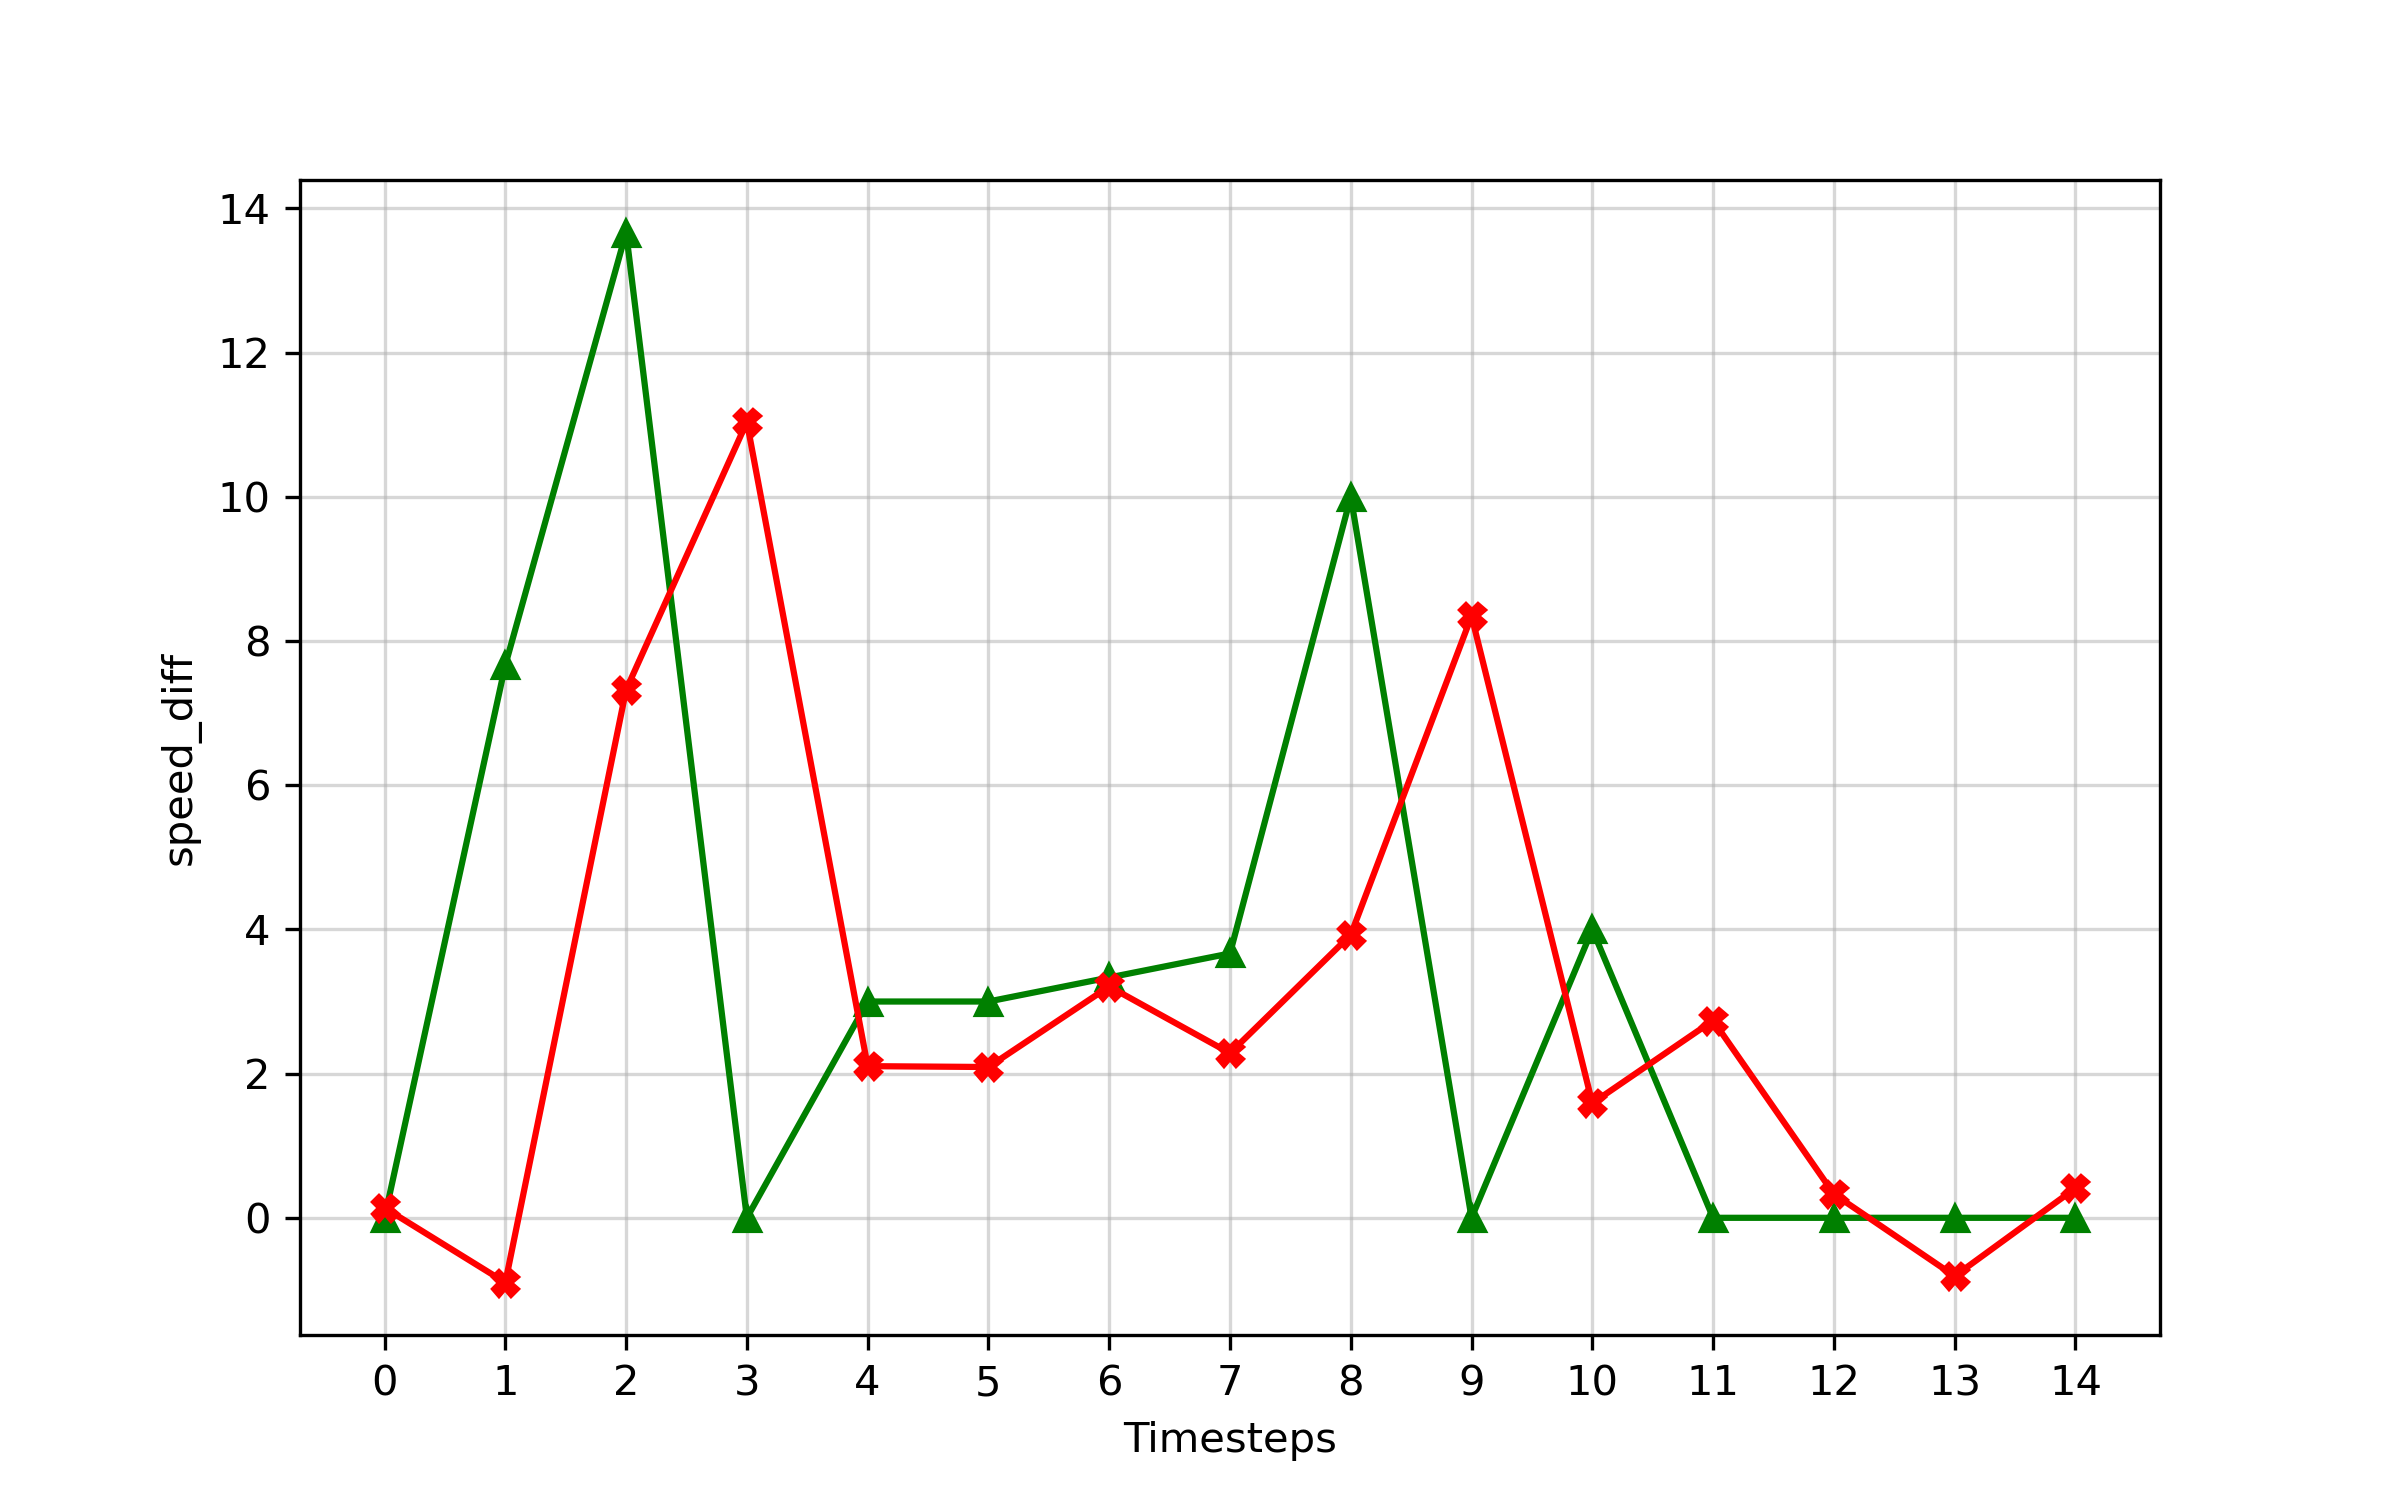
\includegraphics[width=\linewidth]{../private_assets/plot_SpeedDiff_arimax(1,2,3)_predictions_15_crossvalidation_1.png}
}{%
  \caption{Gráfico do modelo \textit{\acrshort{arimax}}(1, 2, 3), 1ª divisão do dataset, com 15 previsões}%
}
\end{floatrow}
\end{figure}

% \begin{table}[h!]
% \centering
% \setlength{\extrarowheight}{4pt}
% \setlength{\tabcolsep}{10pt}
% \begin{tabular}{|c|c|}
% \hline
% \textbf{"Predict"} & \textbf{"speed\_diff"}\\[4pt]
% \hline
% 0.13817744331334328 & 0.0 \\[4pt]
% \thinhline
% -0.8973439961623095&7.66666666666 6 668 \\[4pt]
% \thinhline
% 7.323374989923932&13.66666666666 6 664 \\[4pt]
% \thinhline
% 11.038172786531765 & 0.0 \\[4pt]
% \thinhline
% 2.103461054155741 & 3.0 \\[4pt]
% \thinhline
% 2.091510219928224 & 3.0 \\[4pt]
% \thinhline
% 3.208279408032984&3.33333333333 3 333 \\[4pt]
% \thinhline
% 2.283585816926894&3.666666666666 6 665 \\[4pt]
% \thinhline
% 3.9253583100976295& 1 0.0 \\[4pt]
% \thinhline
% 8.34553662378711 & 0.0 \\[4pt]
% \thinhline
% 1.5898776295568244 & 4.0 \\[4pt]
% \thinhline
% 2.7362308186284343 & 0.0 \\[4pt]
% \thinhline
% 0.3293245341001239 & 0.0 \\[4pt]
% \thinhline
% -0.8090669648652083 & 0.0 \\[4pt]
% \thinhline
% 0.4107963416104033 & 0.0 \\[4pt]
% \hline
% \end{tabular}
% \caption{Previsões do modelo \textit{\acrshort{arimax}}(1, 2, 3), 1ª divisão do dataset, com 15 previsões}
% \end{table}
% 
% \begin{figure}[h!]
% \centering
% 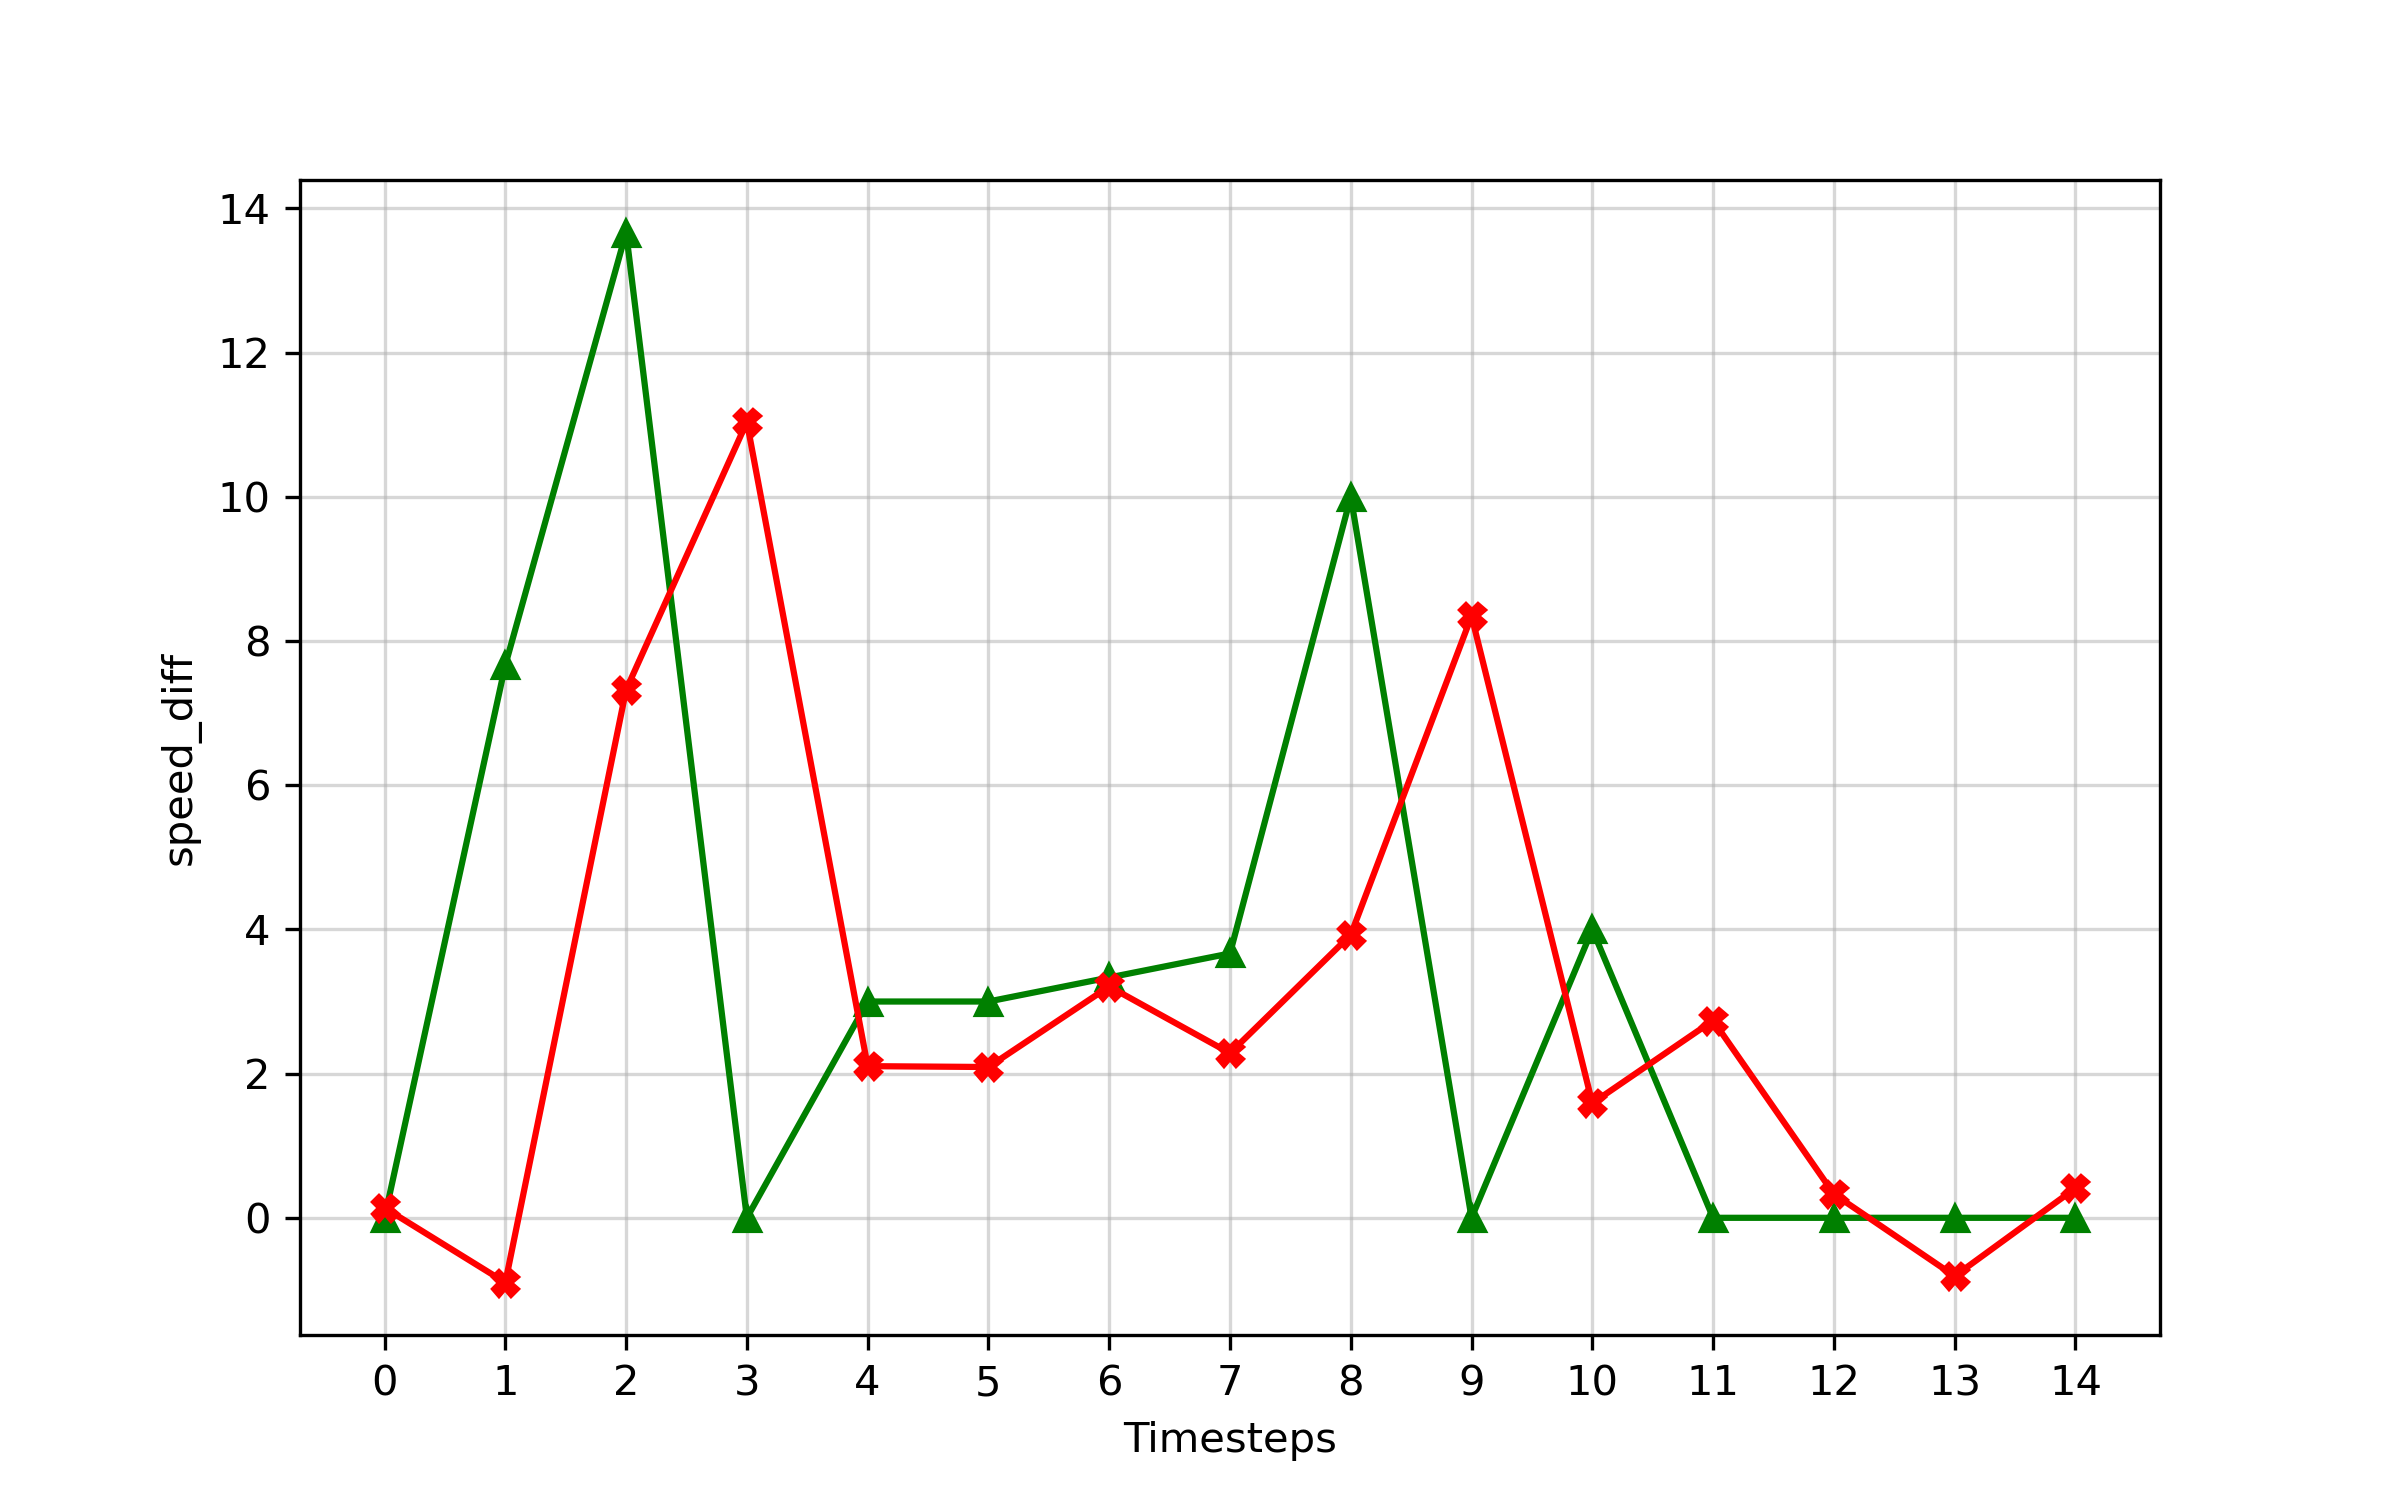
\includegraphics[width=0.9\linewidth]{../private_assets/plot_SpeedDiff_arimax(1,2,3)_predictions_15_crossvalidation_1.png}
% \caption{Gráfico do modelo \textit{\acrshort{arimax}}(1, 2, 3), 1ª divisão do dataset, com 15 previsões}
% \end{figure}

\vspace{1cm}

\begin{figure}[h!]
\begin{floatrow}
\capbtabbox{%
  \setlength{\extrarowheight}{1pt}
  \begin{tabular}{|c|c|} \hline
    \textbf{"Predict"} & \textbf{"speed\_diff"} \\[1pt] \hline
    0.34030661913252236 & 0.0 \\[1pt] \thinhline
    -0.7087282570616925 & 7.666666666666668 \\[1pt] \thinhline
    6.955187335970128 & 13.666666666666664 \\[1pt] \thinhline
    12.210641102705337 & 0.0 \\[1pt] \thinhline
    2.2518274963409595 & 3.0 \\[1pt] \thinhline
    2.236290006499467 & 3.0 \\[1pt] \thinhline
    3.3883287072845674 & 3.333333333333333 \\[1pt] \thinhline
    2.597318025226484 & 3.6666666666666665 \\[1pt] \thinhline
    4.030597662527793 & 10.0 \\[1pt] \thinhline
    8.426346911548624 & 0.0 \\[1pt] \thinhline
    1.8303097185121766 & 4.0 \\[1pt] \thinhline
    2.7647857128428743 & 0.0 \\[1pt] \thinhline
    1.016524698044413 & 0.0 \\[1pt] \thinhline
    -0.7501655819003638 & 0.0 \\[1pt] \thinhline
    0.29871343930839866 & 0.0 \\[1pt] \hline
  \end{tabular}
}{%
  \caption{Previsões do modelo \textit{\acrshort{arima}}(1, 2, 3), 1ª divisão do dataset, com 15 previsões}%
}
\ffigbox{%
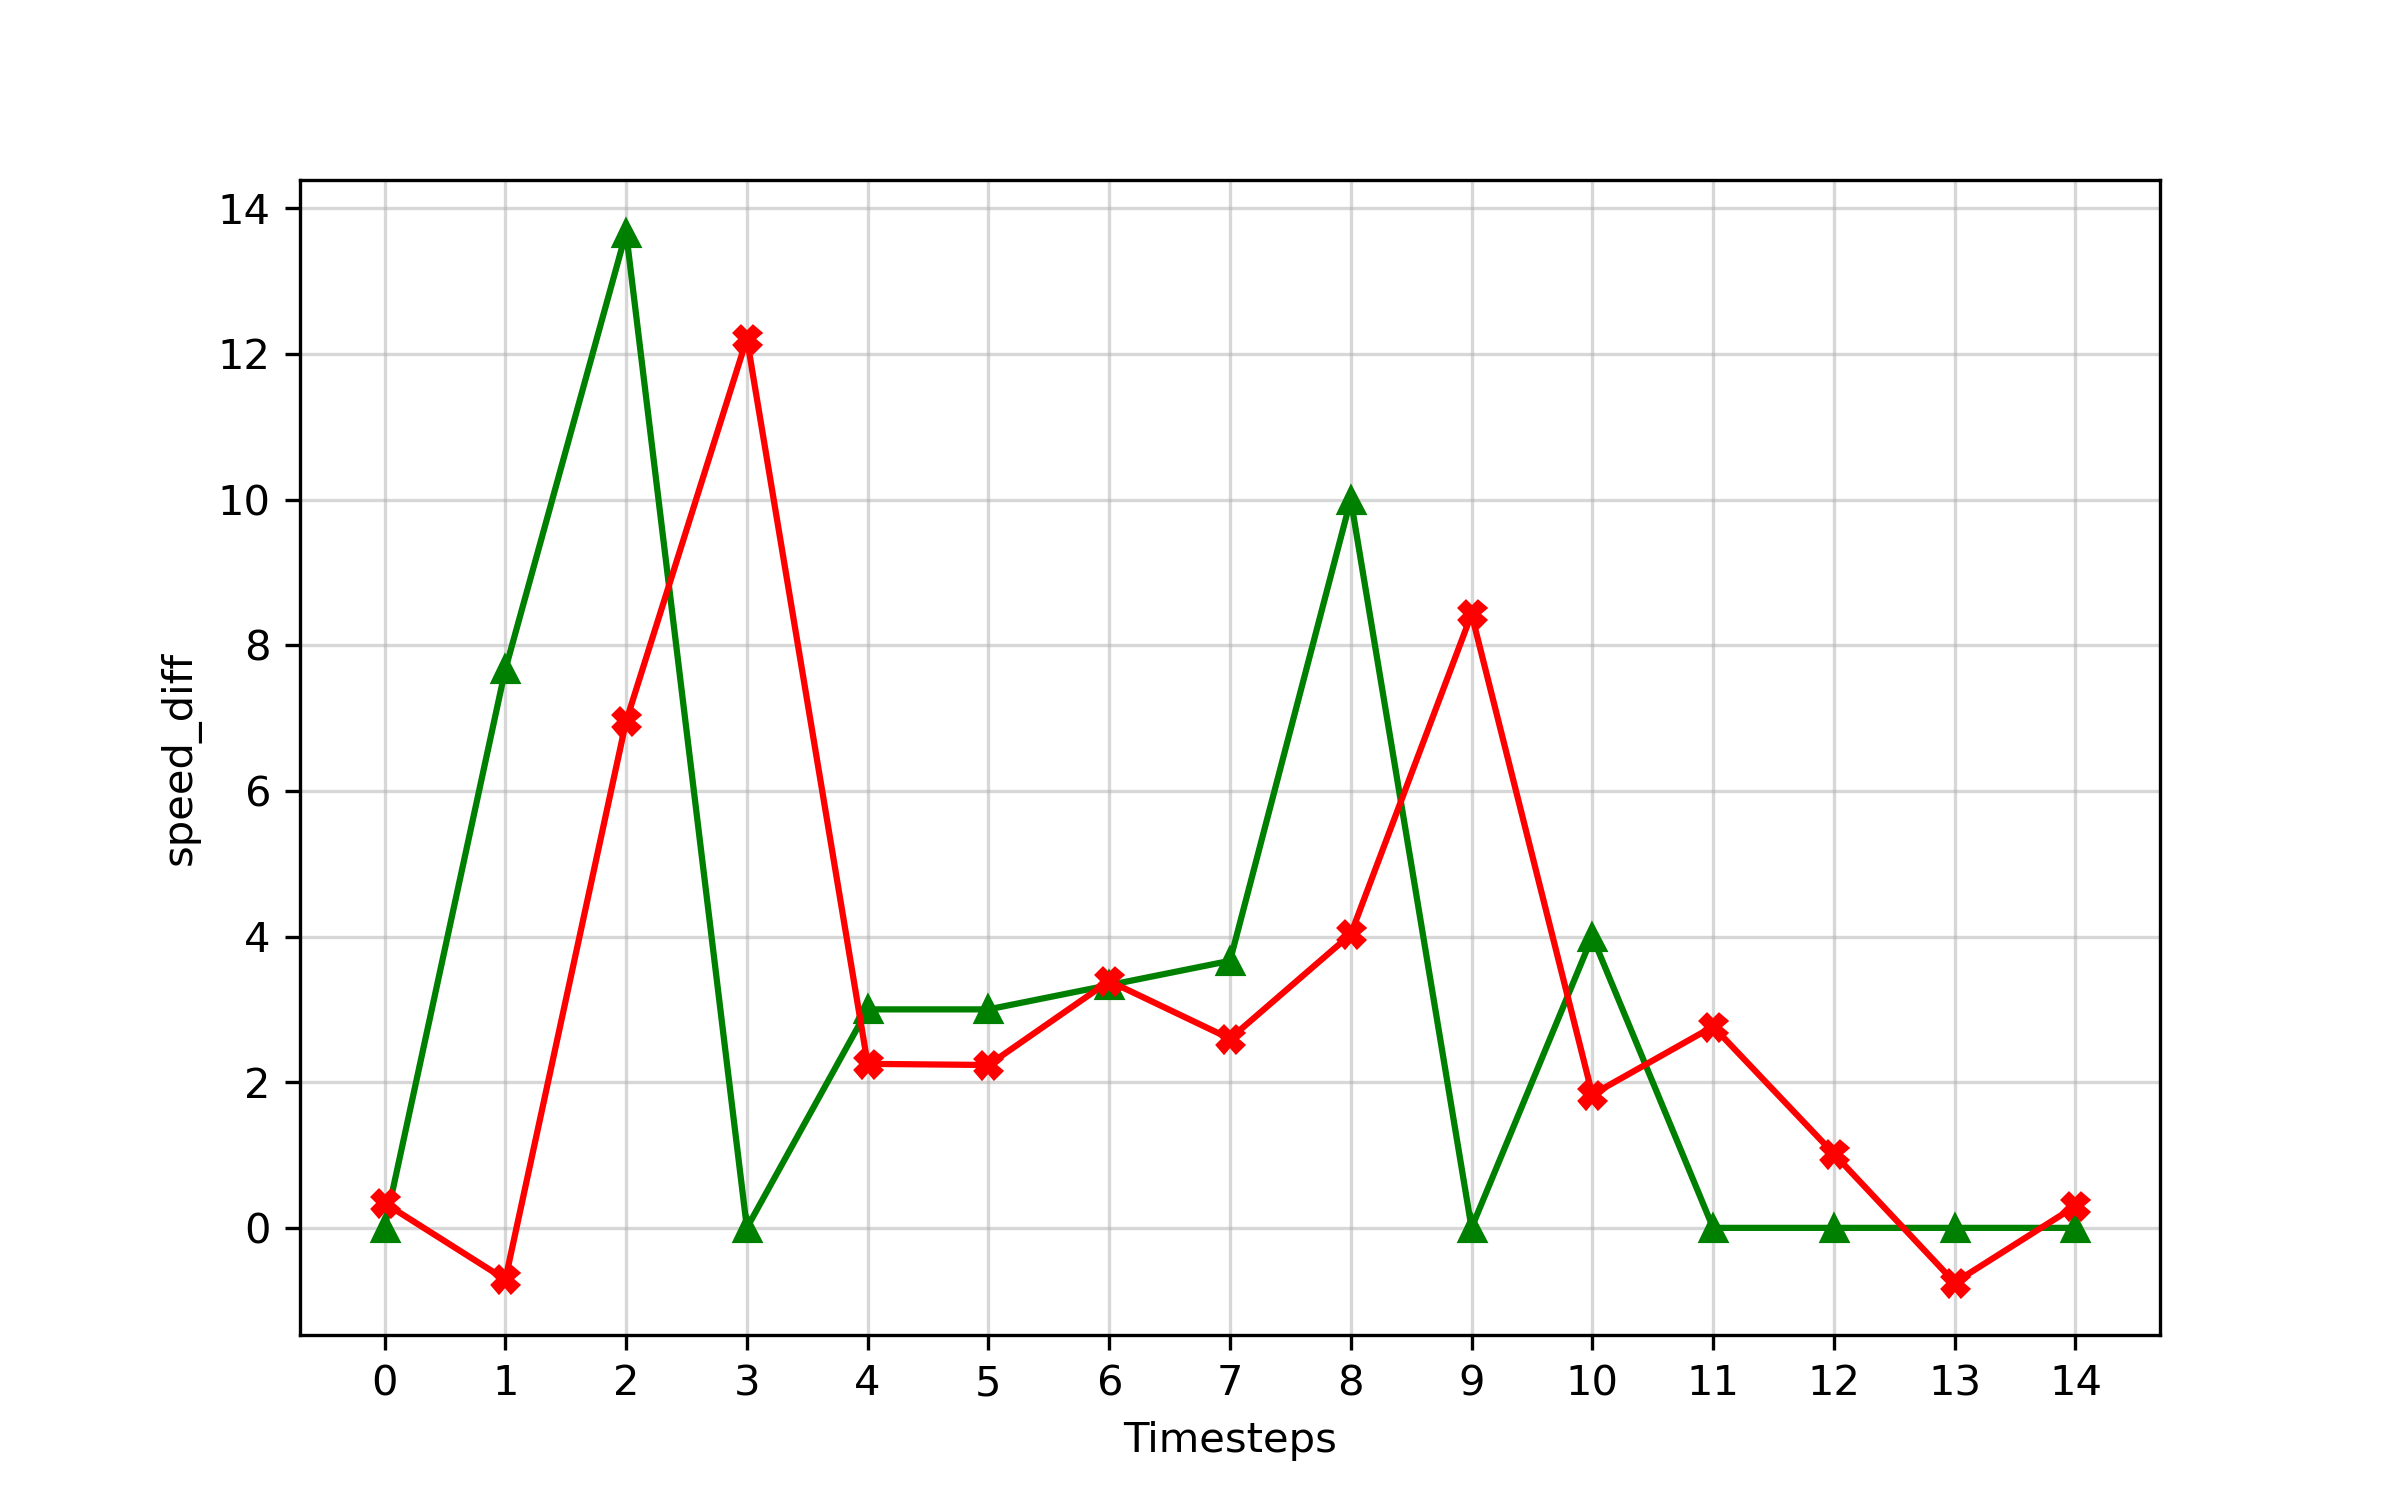
\includegraphics[width=\linewidth]{../private_assets/plot_SpeedDiff_arima(1,2,3)_predictions_15_crossvalidation_1.png}
}{%
  \caption{Gráfico do modelo \textit{\acrshort{arima}}(1, 2, 3), 1ª divisão do dataset, com 15 previsões}%
}
\end{floatrow}
\end{figure}

% \newpage
% \begin{table}[h!]
% \centering
% \setlength{\extrarowheight}{4pt}
% \setlength{\tabcolsep}{10pt}
% \begin{tabular}{|c|c|}
% \hline
% \textbf{"Predict"} & \textbf{"speed\_diff"}\\[4pt]
% \hline
% 0.34030661913252236 & 0.0 \\[4pt]
% \thinhline
% -0.7087282570616925 & 7.666666666666668 \\[4pt]
% \thinhline
% 6.955187335970128 & 13.666666666666664 \\[4pt]
% \thinhline
% 12.210641102705337 & 0.0 \\[4pt]
% \thinhline
% 2.2518274963409595 & 3.0 \\[4pt]
% \thinhline
% 2.236290006499467 & 3.0 \\[4pt]
% \thinhline
% 3.3883287072845674 & 3.333333333333333 \\[4pt]
% \thinhline
% 2.597318025226484 & 3.6666666666666665 \\[4pt]
% \thinhline
% 4.030597662527793 & 10.0 \\[4pt]
% \thinhline
% 8.426346911548624 & 0.0 \\[4pt]
% \thinhline
% 1.8303097185121766 & 4.0 \\[4pt]
% \thinhline
% 2.7647857128428743 & 0.0 \\[4pt]
% \thinhline
% 1.016524698044413 & 0.0 \\[4pt]
% \thinhline
% -0.7501655819003638 & 0.0 \\[4pt]
% \thinhline
% 0.29871343930839866 & 0.0 \\[4pt]
% \hline
% \end{tabular}
% \caption{Previsões do modelo \textit{\acrshort{arima}}(1, 2, 3), 1ª divisão do dataset, com 15 previsões}
% \end{table}

% \begin{figure}[h!]
% \centering
% 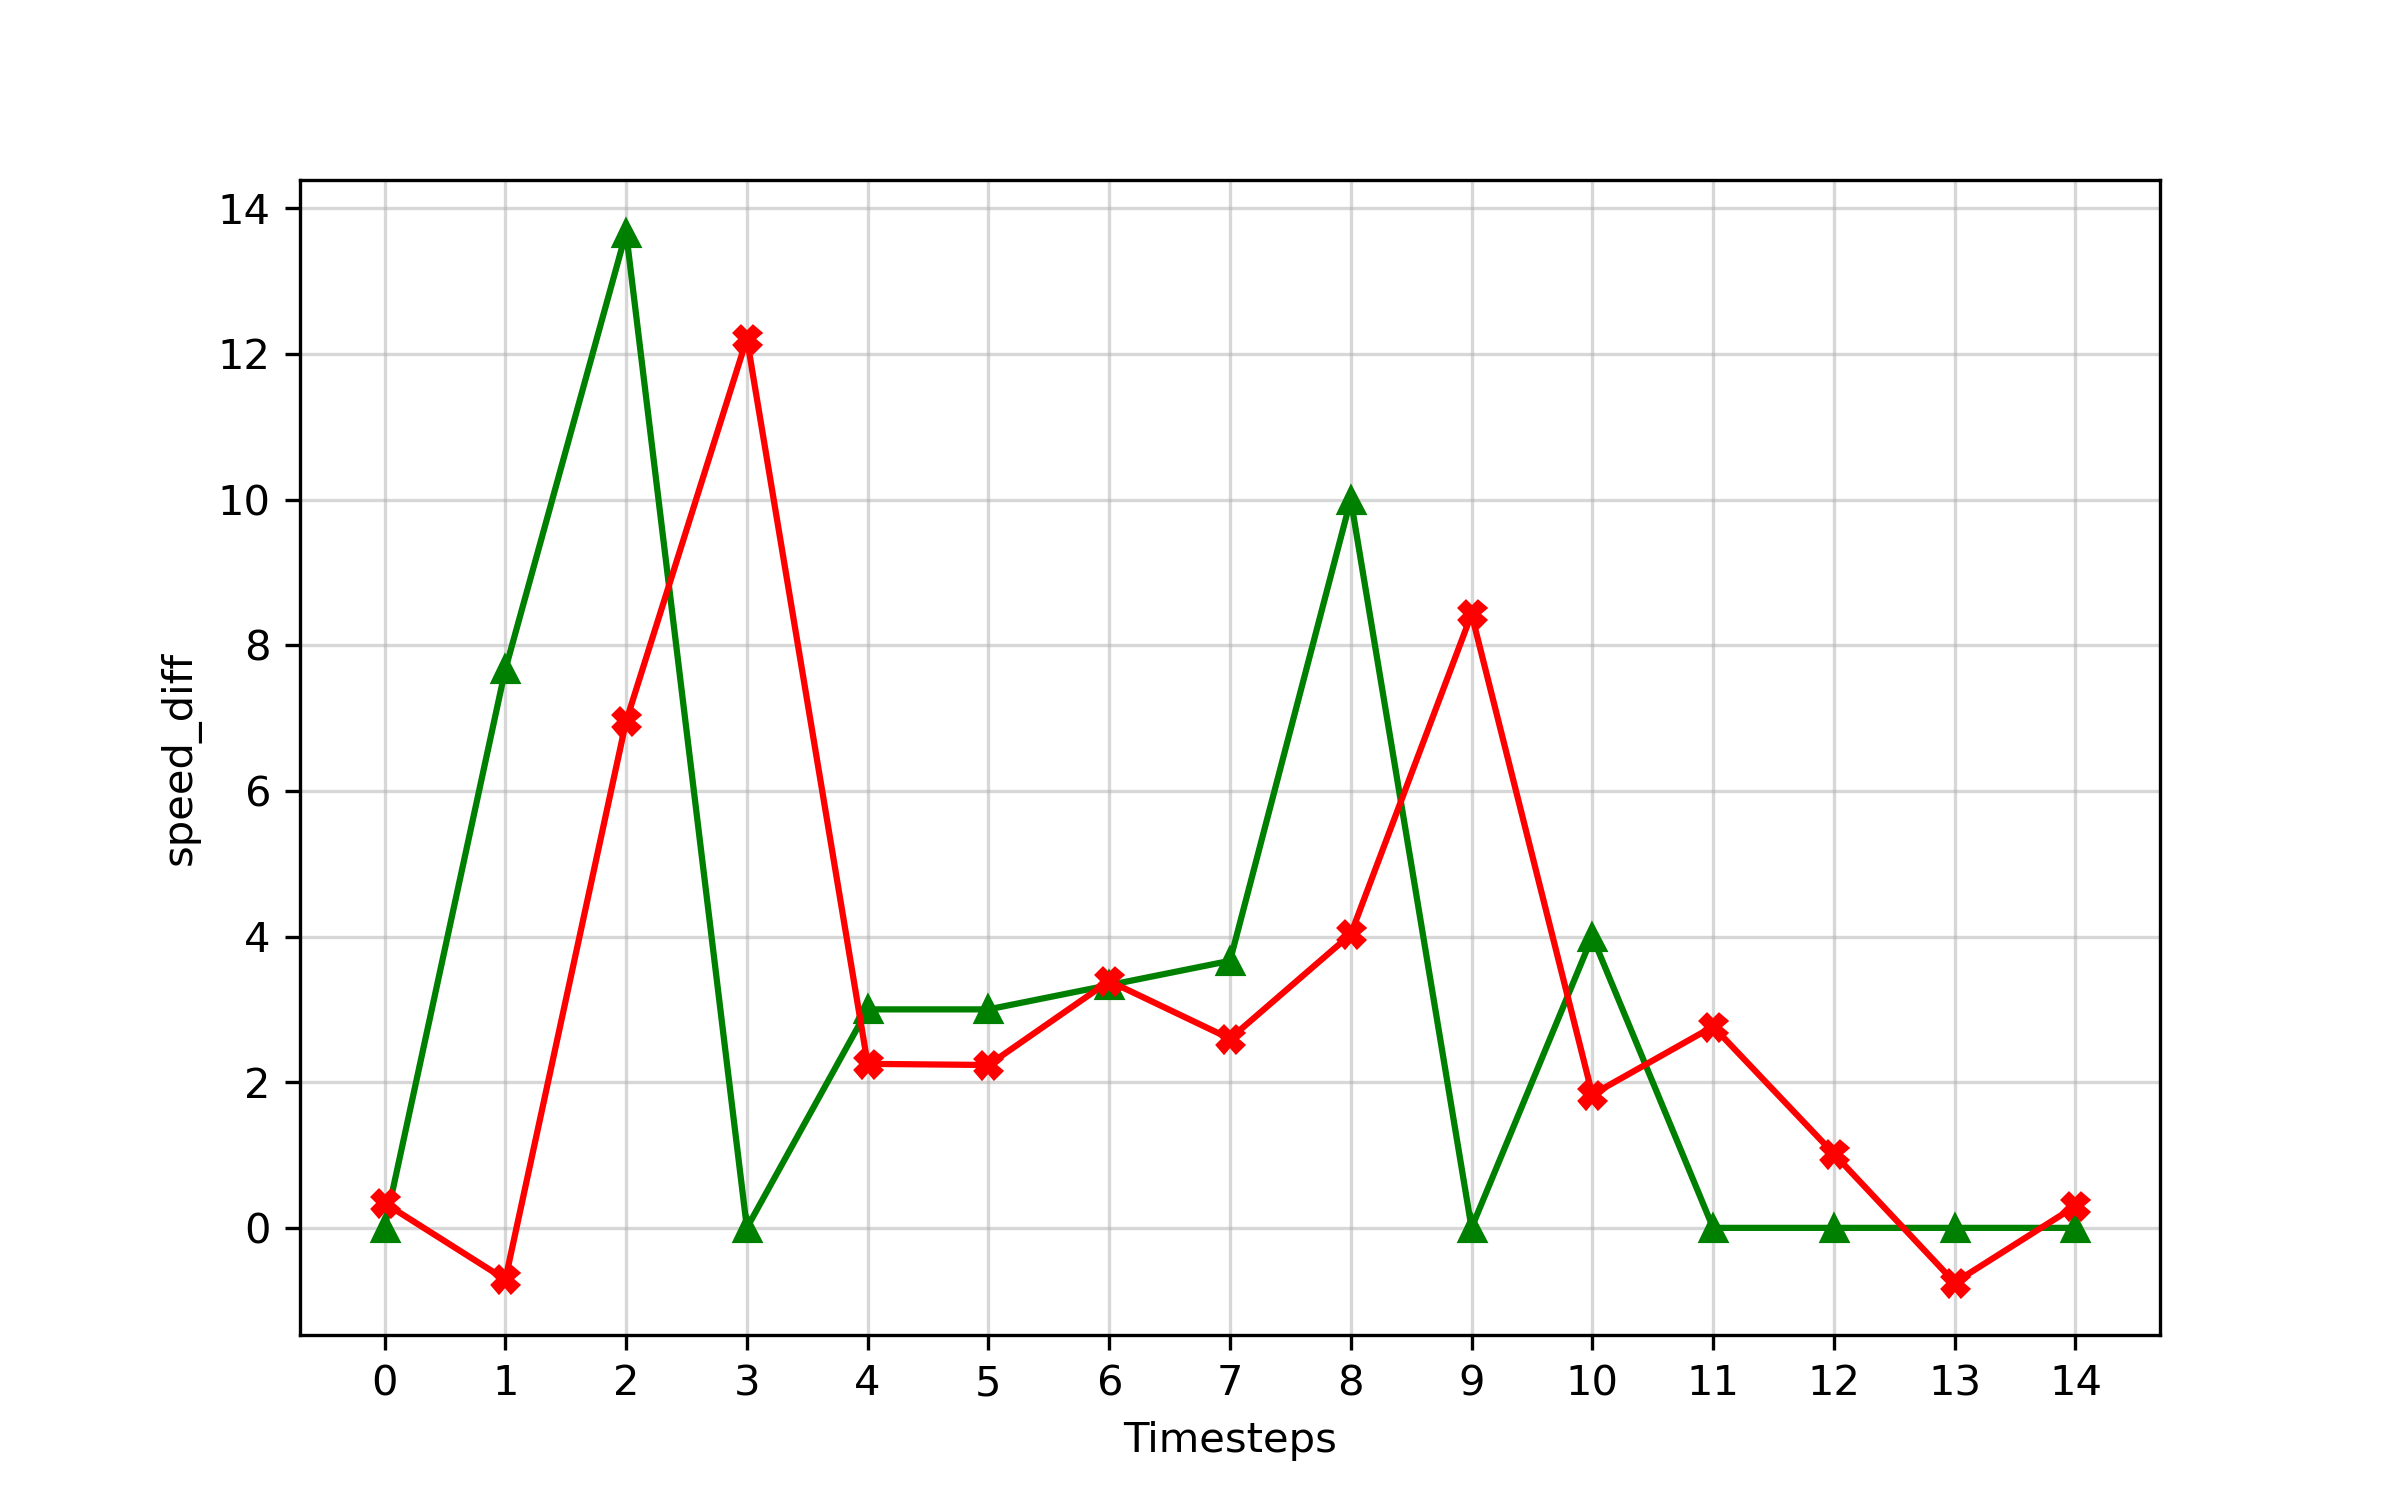
\includegraphics[width=0.9\linewidth]{../private_assets/plot_SpeedDiff_arima(1,2,3)_predictions_15_crossvalidation_1.png}
% \caption{Gráfico do modelo \textit{\acrshort{arima}}(1, 2, 3), 1ª divisão do dataset, com 15 previsões}
% \end{figure}


\newpage
\begin{figure}[h!]
\begin{floatrow}
\capbtabbox{%
  \setlength{\extrarowheight}{1pt}
  \begin{tabular}{|c|c|} \hline
    \textbf{"Predict"} & \textbf{"speed\_diff"} \\[1pt] \hline
    17.942670071265077 & 18.33333333333333 \\[1pt] \thinhline
    17.893110238007367 & 12.0 \\[1pt] \thinhline
    13.32185938423577 & 22.66666666666667 \\[1pt] \thinhline
    20.93896774528977 & 18.666666666666668 \\[1pt] \thinhline
    19.682965507712986 & 23.333333333333336 \\[1pt] \thinhline
    22.402823802743256 & 16.333333333333332 \\[1pt] \thinhline
    18.20671584886394 & 25.66666666666667 \\[1pt] \thinhline
    24.068776185547435 & 32.0 \\[1pt] \thinhline
    31.389219555359038 & 32.66666666666667 \\[1pt] \thinhline
    32.091001235619046 & 21.66666666666667 \\[1pt] \thinhline
    23.538510942114325 & 3.333333333333333 \\[1pt] \thinhline
    5.407697532959148 & 0.0 \\[1pt] \thinhline
    0.9618211695579877 & 0.0 \\[1pt] \thinhline
    -0.5039355197295305 & 0.0 \\[1pt] \thinhline
    0.4393948308917405 & 0.0 \\[1pt] \hline
  \end{tabular}
}{%
  \caption{Previsões do modelo \textit{\acrshort{arima}}(1, 2, 3), 3ª divisão do dataset, com 15 previsões}%
}
\ffigbox{%
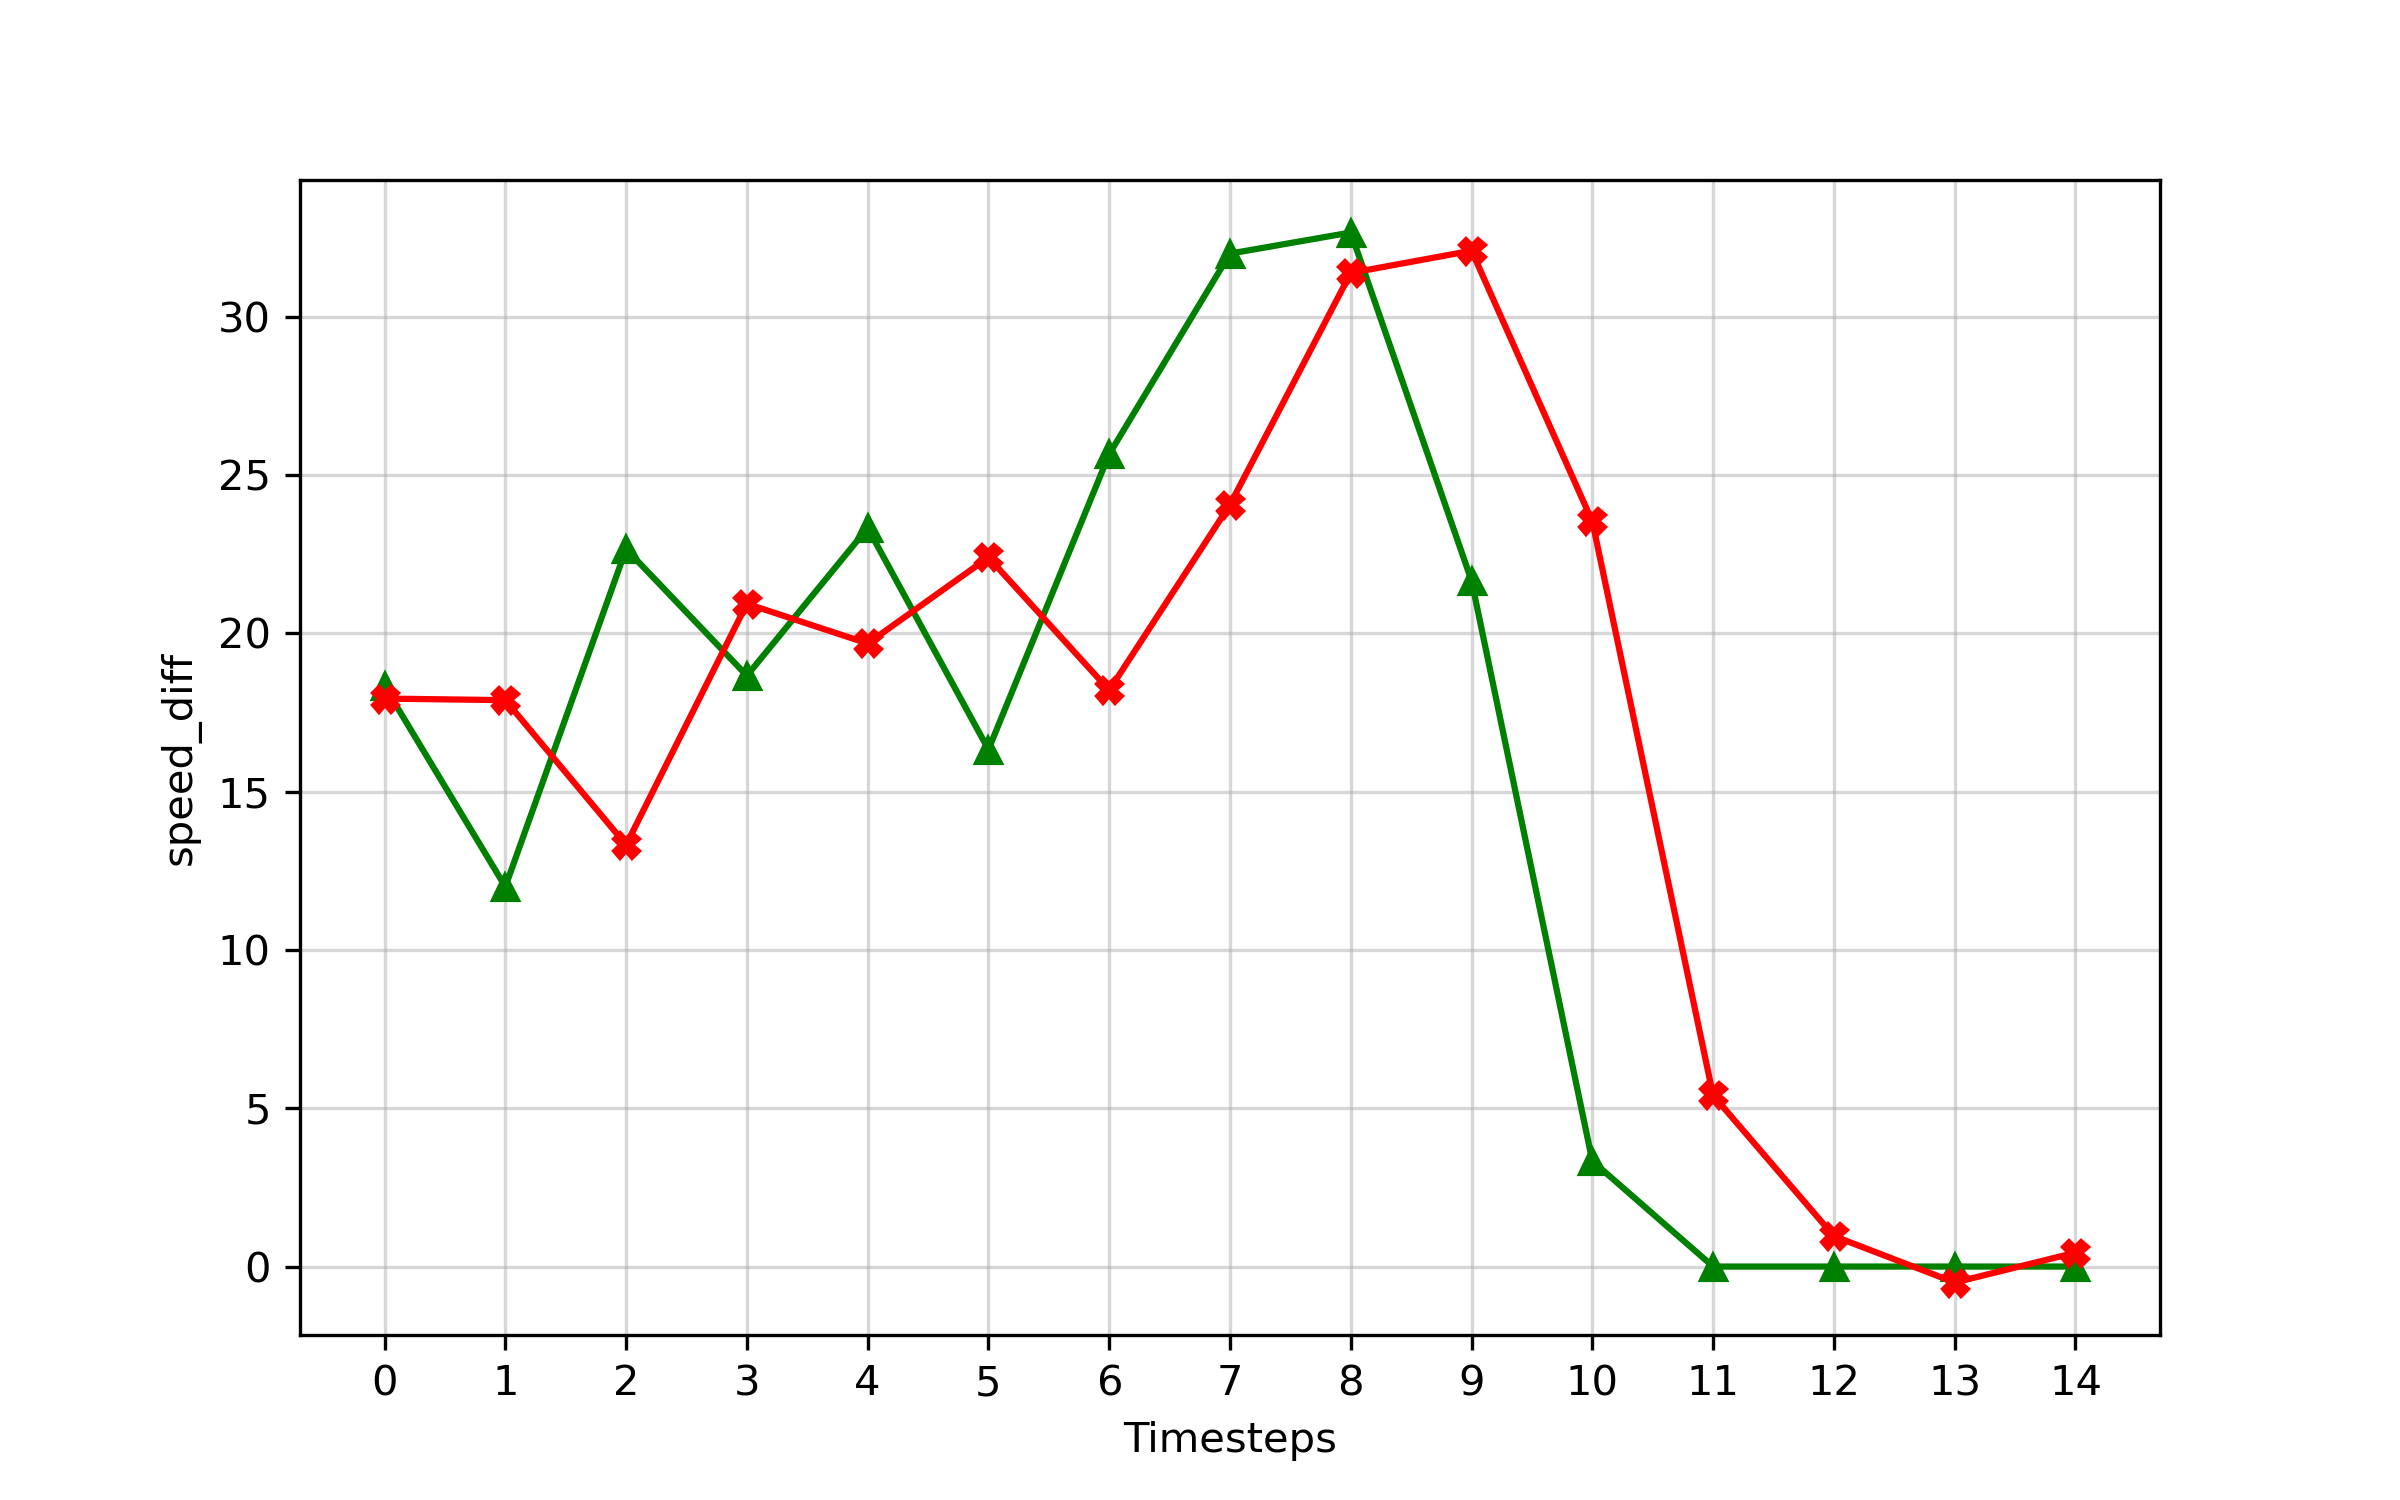
\includegraphics[width=\linewidth]{../private_assets/plot_SpeedDiff_arima(1,2,3)_predictions_15_crossvalidation_3.png}
}{%
  \caption{Gráfico do modelo \textit{\acrshort{arima}}(1, 2, 3), 3ª divisão do dataset, com 15 previsões}%
}
\end{floatrow}
\end{figure}

% \begin{table}[h!]
% \centering
% \setlength{\extrarowheight}{4pt}
% \setlength{\tabcolsep}{10pt}
% \begin{tabular}{|c|c|}
% \hline
% \textbf{"Predict"} & \textbf{"speed\_diff"}\\[4pt]
% \hline
% 17.942670071265077 & 18.33333333333333 \\[4pt]
% \thinhline
% 17.893110238007367 & 12.0 \\[4pt]
% \thinhline
% 13.32185938423577 & 22.66666666666667 \\[4pt]
% \thinhline
% 20.93896774528977 & 18.666666666666668 \\[4pt]
% \thinhline
% 19.682965507712986 & 23.333333333333336 \\[4pt]
% \thinhline
% 22.402823802743256 & 16.333333333333332 \\[4pt]
% \thinhline
% 18.20671584886394 & 25.66666666666667 \\[4pt]
% \thinhline
% 24.068776185547435 & 32.0 \\[4pt]
% \thinhline
% 31.389219555359038 & 32.66666666666667 \\[4pt]
% \thinhline
% 32.091001235619046 & 21.66666666666667 \\[4pt]
% \thinhline
% 23.538510942114325 & 3.333333333333333 \\[4pt]
% \thinhline
% 5.407697532959148 & 0.0 \\[4pt]
% \thinhline
% 0.9618211695579877 & 0.0 \\[4pt]
% \thinhline
% -0.5039355197295305 & 0.0 \\[4pt]
% \thinhline
% 0.4393948308917405 & 0.0 \\[4pt]
% \hline
% \end{tabular}
% \caption{Previsões do modelo \textit{\acrshort{arima}}(1, 2, 3), 3ª divisão do dataset, com 15 previsões}
% \end{table}

% \begin{figure}[h!]
% \centering
% 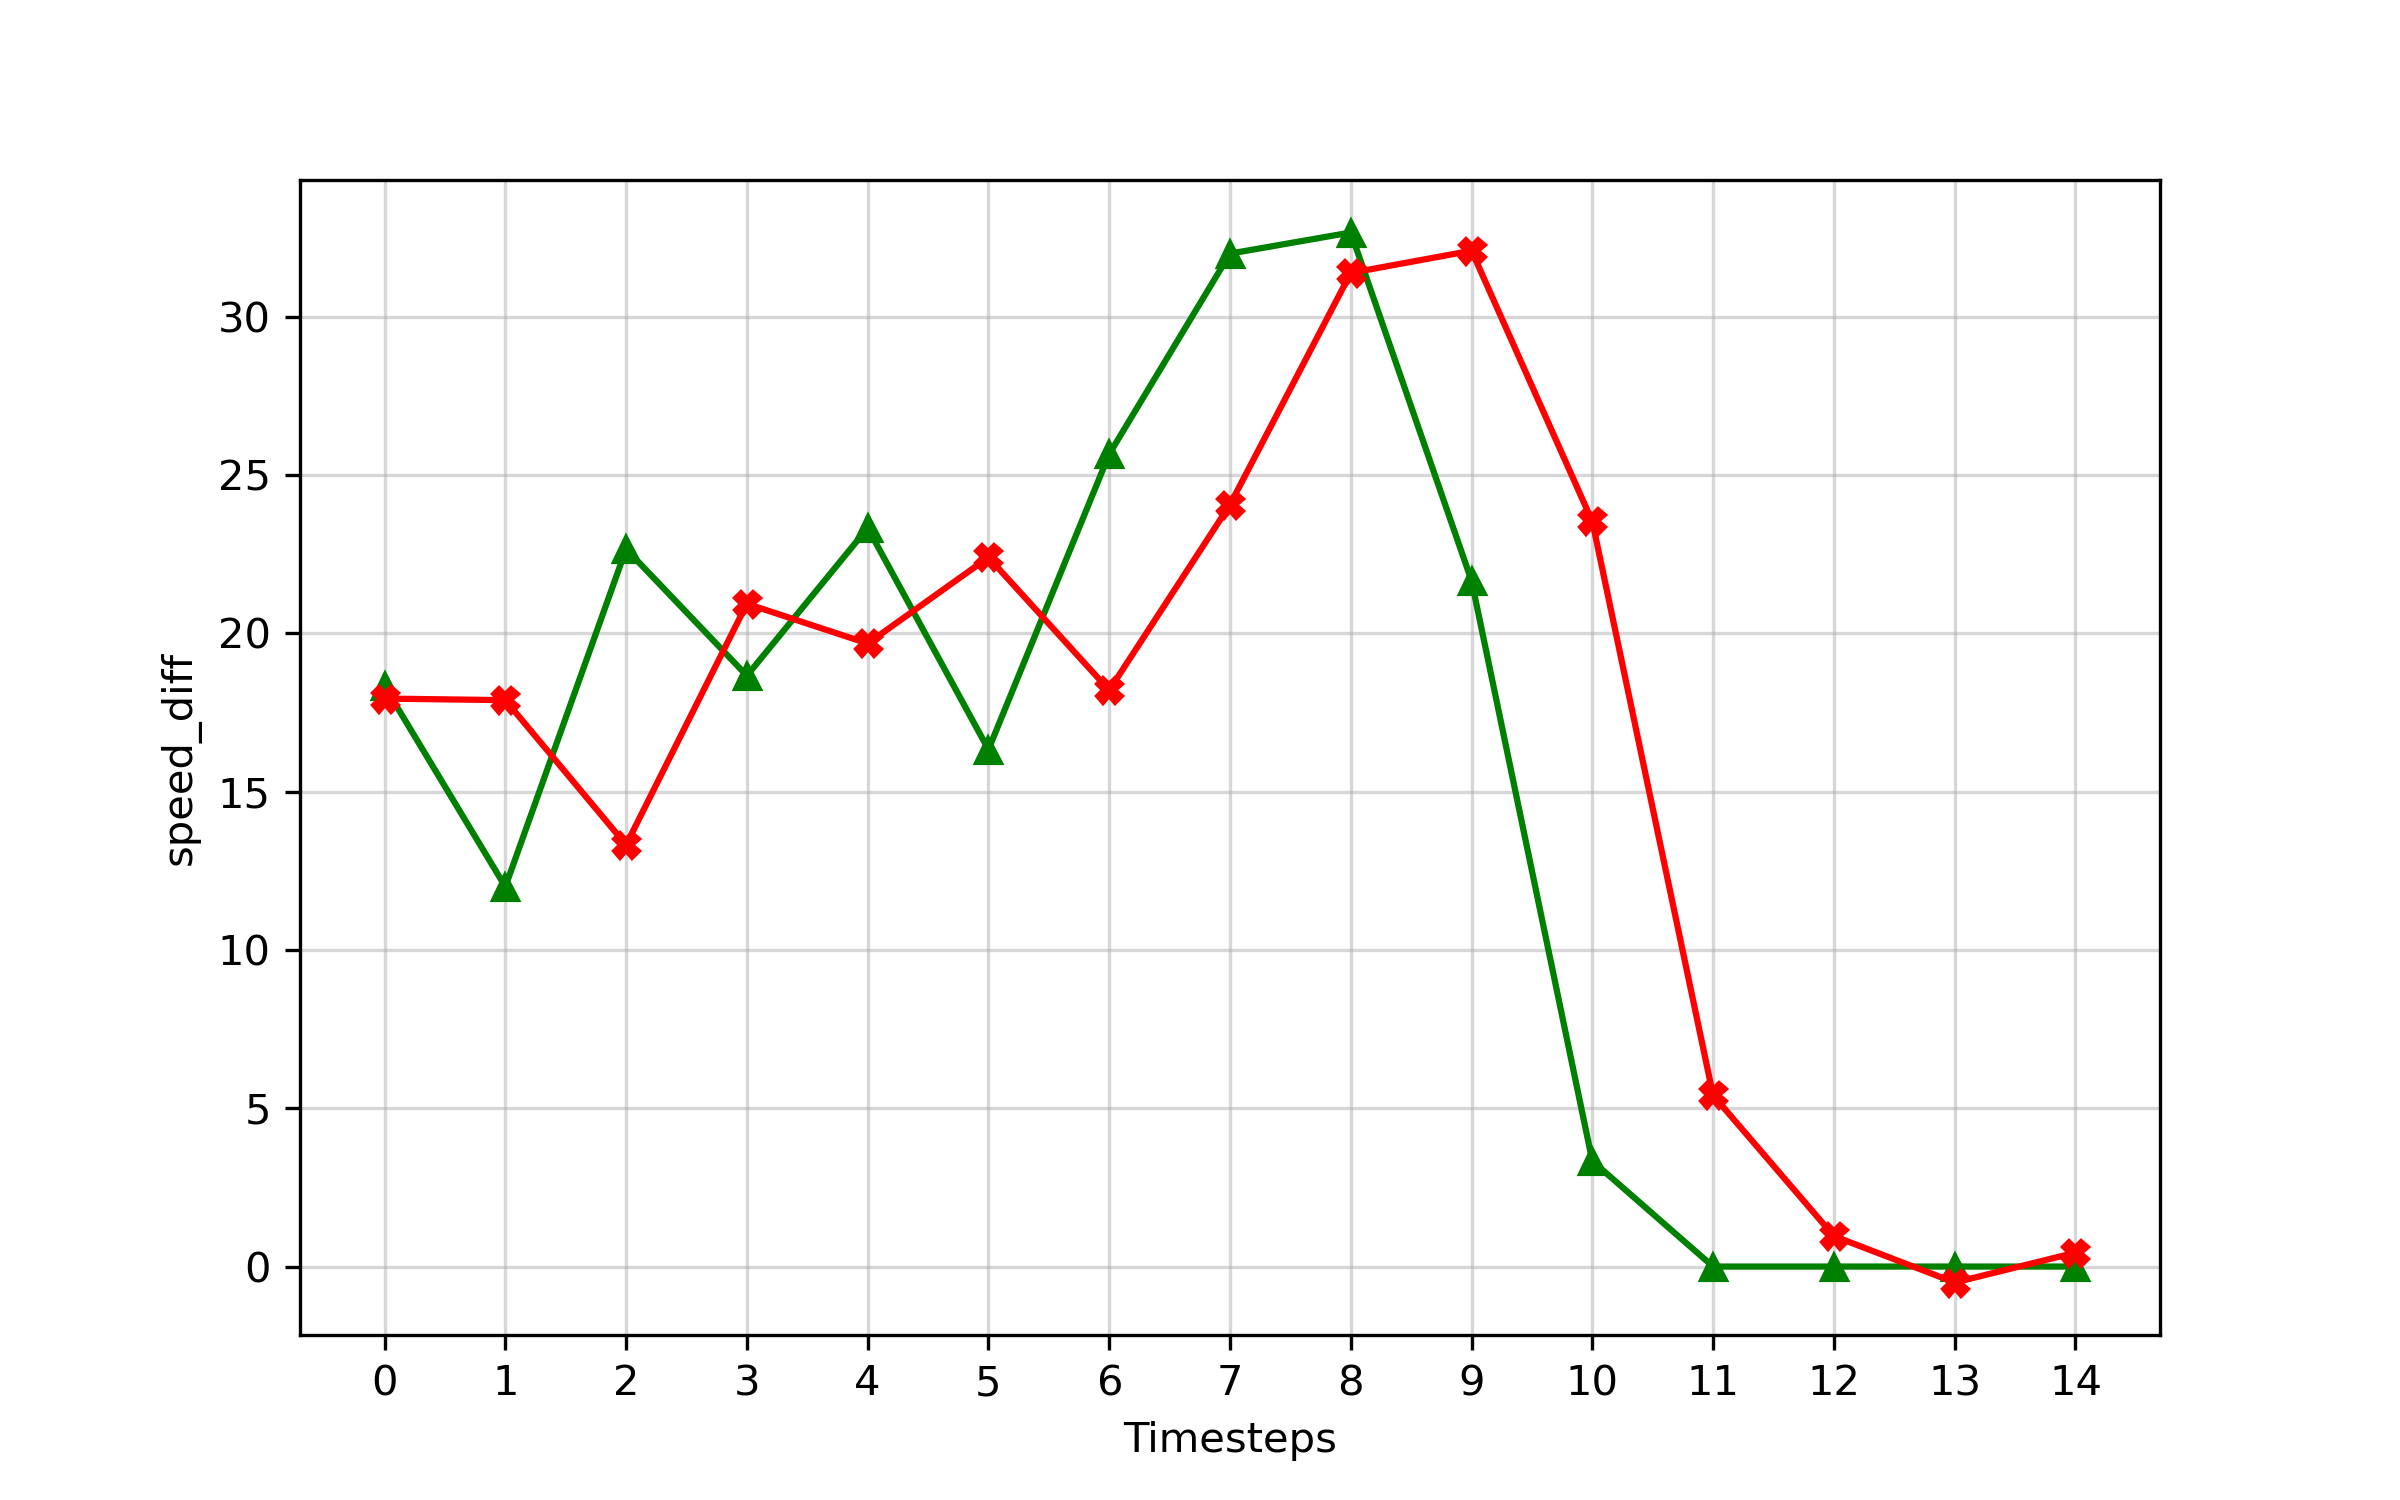
\includegraphics[width=0.9\linewidth]{../private_assets/plot_SpeedDiff_arima(1,2,3)_predictions_15_crossvalidation_3.png}
% \caption{Gráfico do modelo \textit{\acrshort{arima}}(1, 2, 3), 3ª divisão do dataset, com 15 previsões}
% \end{figure}\par

\vspace{1cm}
Em suma, o modelo mais acertivo foi o modelo representado na tabela 5.3 e na figura 5.2.
Posto isto, podemos concluir que a melhor hora para passar na estrada será a hora com maior
diferença de velocidades instantâneas, ou seja, a hora correspondente ao \textit{timestep} número 2.
As piores serão as horas correspondentes aos \textit{timesteps} número 3, 9, e 11 a 14. Analisando o
\textit{\gls{dataset}}, podemos afirmar que a melhor hora será às 12 horas e as piores serão
às 13, às 18 e das 20 até às 23 horas. No entanto, nas horas noturnas é normal não
haver tanto tráfego automóvel, isto é, conclui-se que as piores horas serão às 13 e às 18 horas.

\newpage
\subsection{Caso de Estudo da Quantidade Populacional}
Por outro lado, este conjunto te dados trata-se das medições da quantidade populacional num
quiosque em Nova Iorque. Podem ser apontadas vantagens como: previsão da quantidade de
pessoas num determinado local, o que pode ser uma excelente forma de prevenção da doença
\gls{covid}. Na tabela 5.6 está representado um excerto do conjunto de dados utilizado para
realizar este caso de estudo.\par
\vspace{10pt}
\begin{table}[h!]
\centering
\setlength{\extrarowheight}{5pt}
\setlength{\tabcolsep}{10pt}
\begin{tabular}{|c|c|c|c|c|}
\hline
\textbf{"date"} & \textbf{"wifi status"} & \textbf{"temp"} & \textbf{"precipitation"} & \textbf{"census"} \\[5pt]
\hline
01/01/2016 & up & -6 & 0 & 4092 \\[5pt]
\thinhline
02/01/2016 & up & 2 & 0 & 3807 \\[5pt]
\thinhline
03/01/2016 & up & 2 & 0 & 3208 \\[5pt]
\thinhline
04/01/2016 & up & -4 & 0 & 1057 \\[5pt]
\thinhline
05/01/2016 & up & 2 & 0 & 3302 \\[5pt]
\thinhline
06/01/2016 & up & 2 & 0 & 3761 \\[5pt]
\thinhline
07/01/2016 & up & 4 & 0 & 2964 \\[5pt]
\hline
\end{tabular}
\caption{Excerto do \textit{\gls{dataset}} de quantidade populacional}
\end{table}

Na figura 5.5 pode ser visualizado um diagrama de extremos e quartis do
\textit{\gls{dataset}} de quantidade populacional relativo ao ano de 2018.\par
\begin{figure}[h!]
\centering
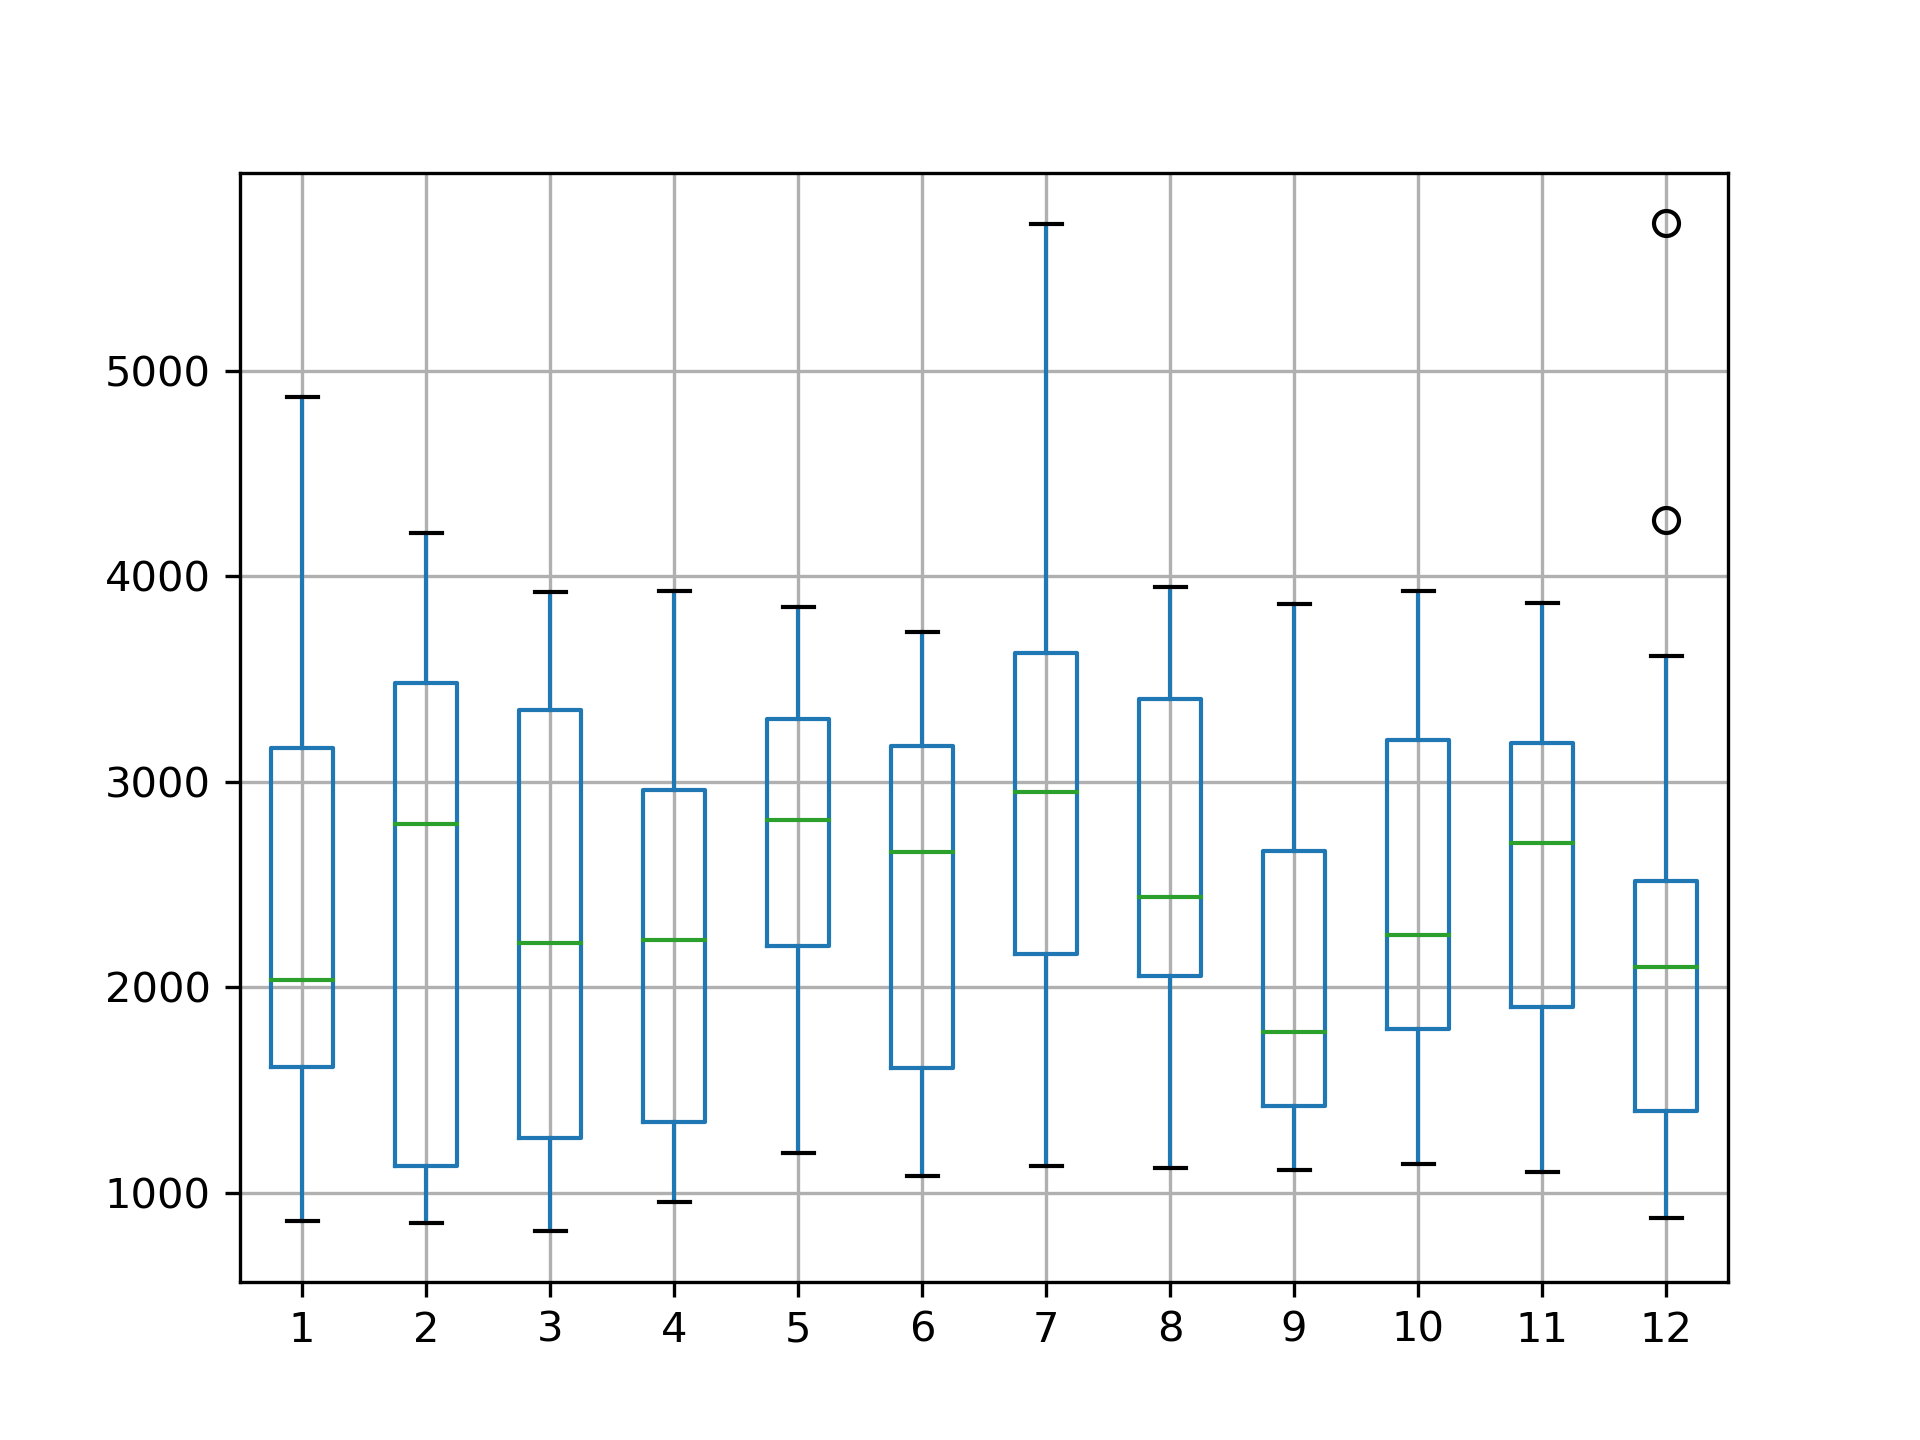
\includegraphics[width=0.8\linewidth]{../private_assets/boxplot_census_2018_dataset.png}
\caption{Diagrama de extremos e quartis do ano de 2018 do \textit{\gls{dataset}} de quantidade populacional}
\end{figure}

Algumas perguntas que visam ser respondidas no final deste caso de estudo são:
\begin{itemize}
    \item Qual o melhor dia do mês para ir ao quiosque?
    \item Qual o pior dia do mês para ir ao quiosque?
\end{itemize}\par
Para esta série temporal, foram realizadas as \textit{grid searches} da seguinte forma:\par
\begin{enumerate}[label=\roman*)]
    \item Correr \textit{\acrshort{arima}}(p, d, q) com:
    \begin{itemize}
        \item p entre 1 e 5;
        \item d entre 0 e 2;
        \item q entre 0 e 2.
    \end{itemize}
    \item Escolher 4 melhores configurações do \textit{\acrshort{arima}};
    \item Correr \textit{\acrshort{sarima}(p, d, q)(P, D, Q, S)} com as 4 melhores
    configurações dos primeiros parâmetros definidos no passo anterior;
    \item Escolher 2 melhores conjuntos dos parâmetros do \textit{\acrshort{sarima}}.
\end{enumerate}\par
Escolher as variáveis exógenas dos modelos \textit{\acrshort{arimax}} e
\textit{\acrshort{sarimax}} é um pouco mais complexo e exige uma compreensão e estudo do
\textit{\gls{dataset}} em si. Se não for escolhida nenuma variável o modelo não faz sentido
ser executado. Por outro lado, caso seja escolhidas muitas variáveis o modelo ou demora uma
eternidade a terminar ou não retorna resultados nenhuns. Isto significa que, para escolher
estas variáveis é necessário ir testanto as que dão melhores resultados e porquê e,
finalmente, quando estiver a análise feita, juntá-las às configurações iniciais dos
algoritmos.\par
Para terminar, tendo já sido escolhidas as melhores configurações dos dois tipos de
parâmetros, correm-se os modelos todos com as configurações acima descritas. Deste modo, nos
modelos \textit{\acrshort{arima}} e \textit{\acrshort{arimax}} existem 4 possibilidades de
teste e nos modelos \textit{\acrshort{sarima}} e \textit{\acrshort{sarimax}} existem 8
possibilidades. Isto ajuda imenso na previsão de daodos, porque com a utilização das
pesquisas em grelha, não é necessário correr todas as cofigurações para todos os modelos,
ou seja, demora mesmo muito menos tempo.\par

\newpage
\begin{table}[h!]
\centering
\setlength{\extrarowheight}{5pt}
\begin{tabular}{|c|c|c|c|}
\hline
\textbf{"Model"} & \textbf{"MAE"} & \textbf{"MSE"} & \textbf{"RMSE"} \\[5pt]
\hline
"ARIMA(1,2,0)\_20" & 431.4058281994794 & 294362.5316925172 & 542.5518700479404 \\[5pt]
\thinhline
"ARIMA(3,2,0)\_20" & 436.2527892941756 & 327546.80919104733 & 572.3170530318378 \\[5pt]
\thinhline
"ARIMA(2,2,0)\_20" & 470.73536627219164 & 339518.96987558715 & 582.6825635589134 \\[5pt]
\thinhline
"ARIMA(4,2,0)\_20" & 463.6572887631079 & 397280.74748587905 & 630.3021081083888 \\[5pt]
\thinhline
"ARIMA(5,2,0)\_20" & 481.2747052602357 & 463843.7919440161 & 681.0607843239957 \\[5pt]
\thinhline
"ARIMA(1,1,0)\_20" & 450.17960473297154 & 464377.9889890727 & 681.4528516259013 \\[5pt]
\hline
\end{tabular}
\caption{Excerto sumário de resultados da \textit{\gls{grid search}} do segundo caso de estudo}
\end{table}\par

A tabela 5.7 representa o sumário de resultados da \textit{\gls{grid search}} do dataset da
quantidade populacional.\par
Conclui-se assim que os 3 melhores modelos testados para este \textit{\gls{dataset}} foram:\\[10pt]
\indent\textit{\acrshort{arima}}(1, 2, 0), sem validação cruzada, com 20 previsões.
Representado na tabela 5.8 e na figura 5.6;\\
\indent\textit{\acrshort{arima}}(3, 2, 0), sem validação cruzada, com 20 previsões.
Representado na tabela 5.9 e na figura 5.7;\\
\indent\textit{\acrshort{arima}}(2, 2, 0), sem validação cruzada, com 20 previsões.
Representado na tabela 5.10 e na figura 5.8;\\[10pt]
\enlargethispage{\baselineskip}

\newpage
\newgeometry{top=2cm, bottom=2cm}

\begin{figure}[h!]
\begin{floatrow}
\capbtabbox{%
  \begin{tabular}{|c|c|} \hline
    \textbf{"Predict"} & \textbf{"census"} \\ \hline
    2071.4553305007325 & 1000.0 \\ \thinhline
    991.9236886020411 & 877.0000000000001 \\ \thinhline
    322.59086790167925 & 1126.0 \\ \thinhline
    1150.7135663993647 & 958.0 \\ \thinhline
    1042.8648699235348 & 1128.0 \\ \thinhline
    1094.1752495844441 & 1509.0 \\ \thinhline
    1763.3997606287378 & 2474.0 \\ \thinhline
    3087.421245832234 & 1928.9999999999998 \\ \thinhline
    2298.294797507882 & 2560.0 \\ \thinhline
    2480.2184224343887 & 2126.0000000000005 \\ \thinhline
    2337.123922709361 & 2398.0 \\ \thinhline
    2243.3011173547725 & 1834.0000000000002 \\ \thinhline
    1776.2634968906202 & 2094.0 \\ \thinhline
    1855.7064948556406 & 2116.0000000000005 \\ \thinhline
    2282.8257530269984 & 2089.0 \\ \thinhline
    2092.242524019219 & 2246.0000000000005 \\ \thinhline
    2292.346701629985 & 2384.0 \\ \thinhline
    2534.3085052761926 & 3011.0 \\ \thinhline
    3343.248508896108 & 4274.0 \\ \thinhline
    5154.176860337541 & 5720.0 \\ \hline
  \end{tabular}
}{%
  \caption{Previsões do modelo \textit{\acrshort{arima}}(1, 2, 0), com 20 previsões}%
}
\ffigbox{%
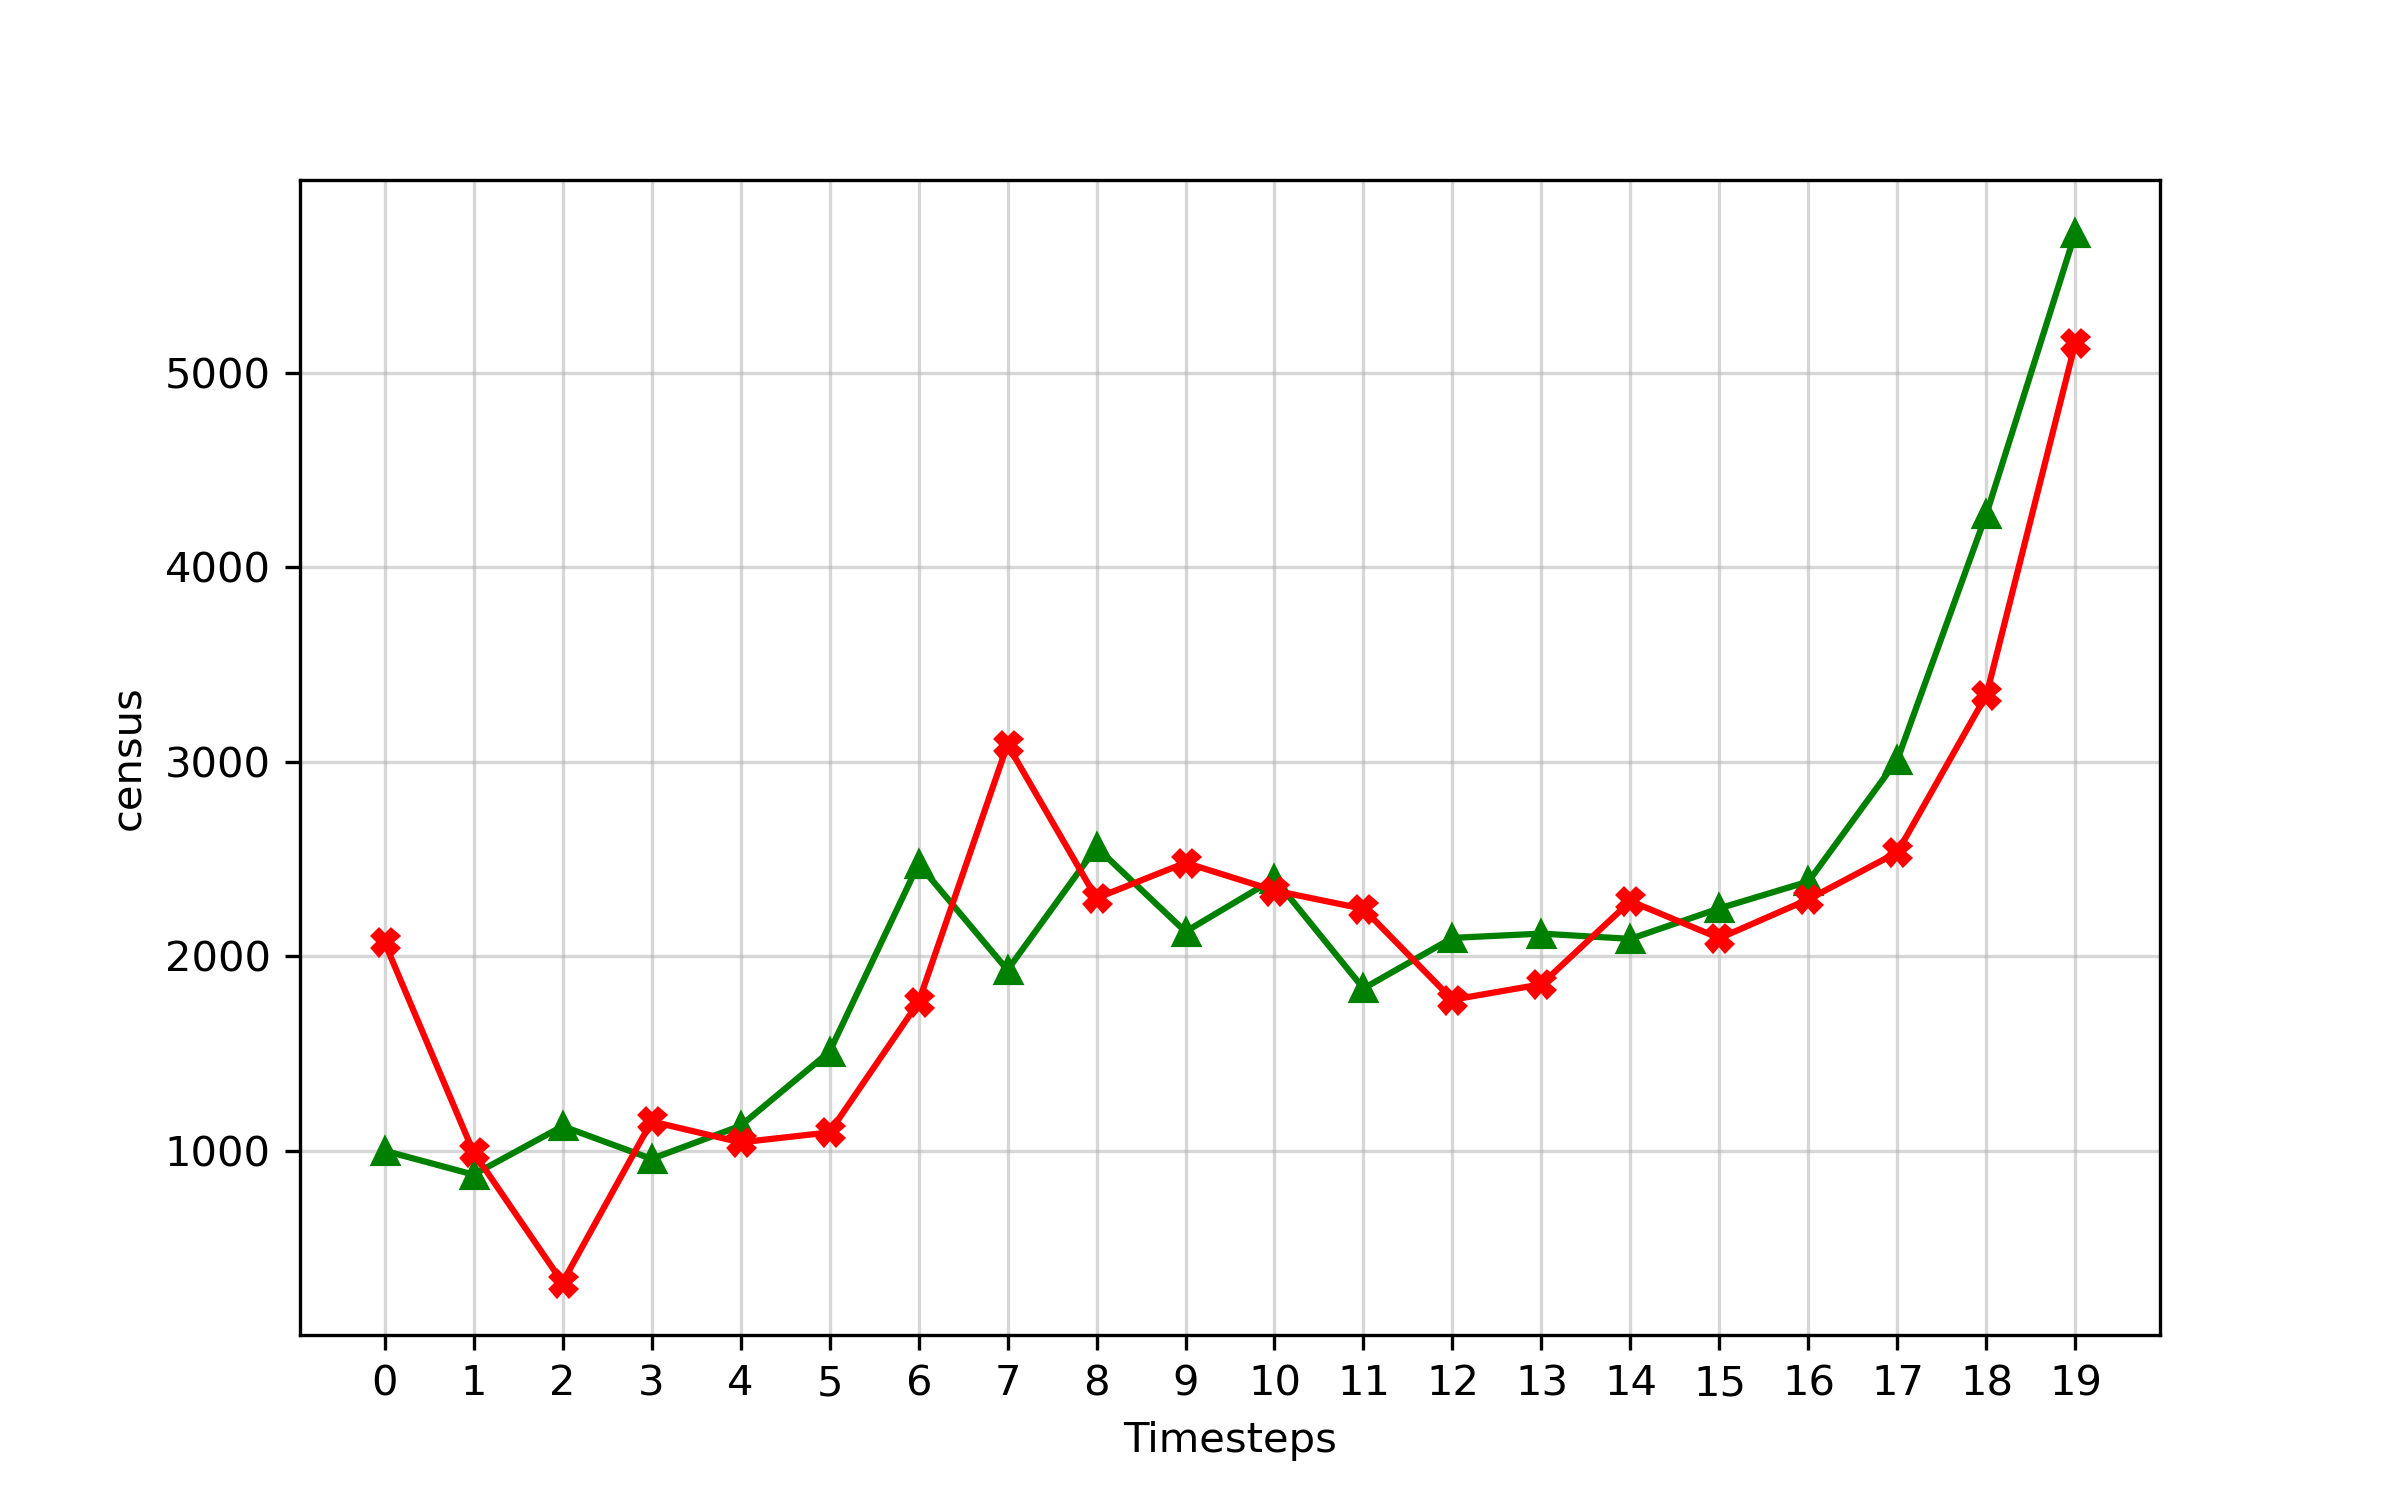
\includegraphics[width=\linewidth]{../private_assets/plot_Census_arima(1,2,0)_predictions_20.png}
}{%
  \caption{Gráfico do modelo \textit{\acrshort{arima}}(1, 2, 0), com 20 previsões}%
}
\end{floatrow}
\end{figure}

% \begin{table}[h!]
% \centering
% \setlength{\extrarowheight}{2pt}
% \setlength{\tabcolsep}{10pt}
% \begin{tabular}{|c|c|}
% \hline
% \textbf{"Predict"} & \textbf{"speed\_diff"}\\[2pt]
% \hline
% 2071.4553305007325 & 1000.0 \\[2pt]
% \thinhline
% 991.9236886020411 & 877.0000000000001 \\[2pt]
% \thinhline
% 322.59086790167925 & 1126.0 \\[2pt]
% \thinhline
% 1150.7135663993647 & 958.0 \\[2pt]
% \thinhline
% 1042.8648699235348 & 1128.0 \\[2pt]
% \thinhline
% 1094.1752495844441 & 1509.0 \\[2pt]
% \thinhline
% 1763.3997606287378 & 2474.0 \\[2pt]
% \thinhline
% 3087.421245832234 & 1928.9999999999998 \\[2pt]
% \thinhline
% 2298.294797507882 & 2560.0 \\[2pt]
% \thinhline
% 2480.2184224343887 & 2126.0000000000005 \\[2pt]
% \thinhline
% 2337.123922709361 & 2398.0 \\[2pt]
% \thinhline
% 2243.3011173547725 & 1834.0000000000002 \\[2pt]
% \thinhline
% 1776.2634968906202 & 2094.0 \\[2pt]
% \thinhline
% 1855.7064948556406 & 2116.0000000000005 \\[2pt]
% \thinhline
% 2282.8257530269984 & 2089.0 \\[2pt]
% \thinhline
% 2092.242524019219 & 2246.0000000000005 \\[2pt]
% \thinhline
% 2292.346701629985 & 2384.0 \\[2pt]
% \thinhline
% 2534.3085052761926 & 3011.0 \\[2pt]
% \thinhline
% 3343.248508896108 & 4274.0 \\[2pt]
% \thinhline
% 5154.176860337541 & 5720.0 \\[2pt]
% \hline
% \end{tabular}
% \caption{Previsões do modelo \textit{\acrshort{arima}}(1, 2, 0), com 20 previsões}
% \end{table}

% \begin{figure}[h!]
% \centering
% 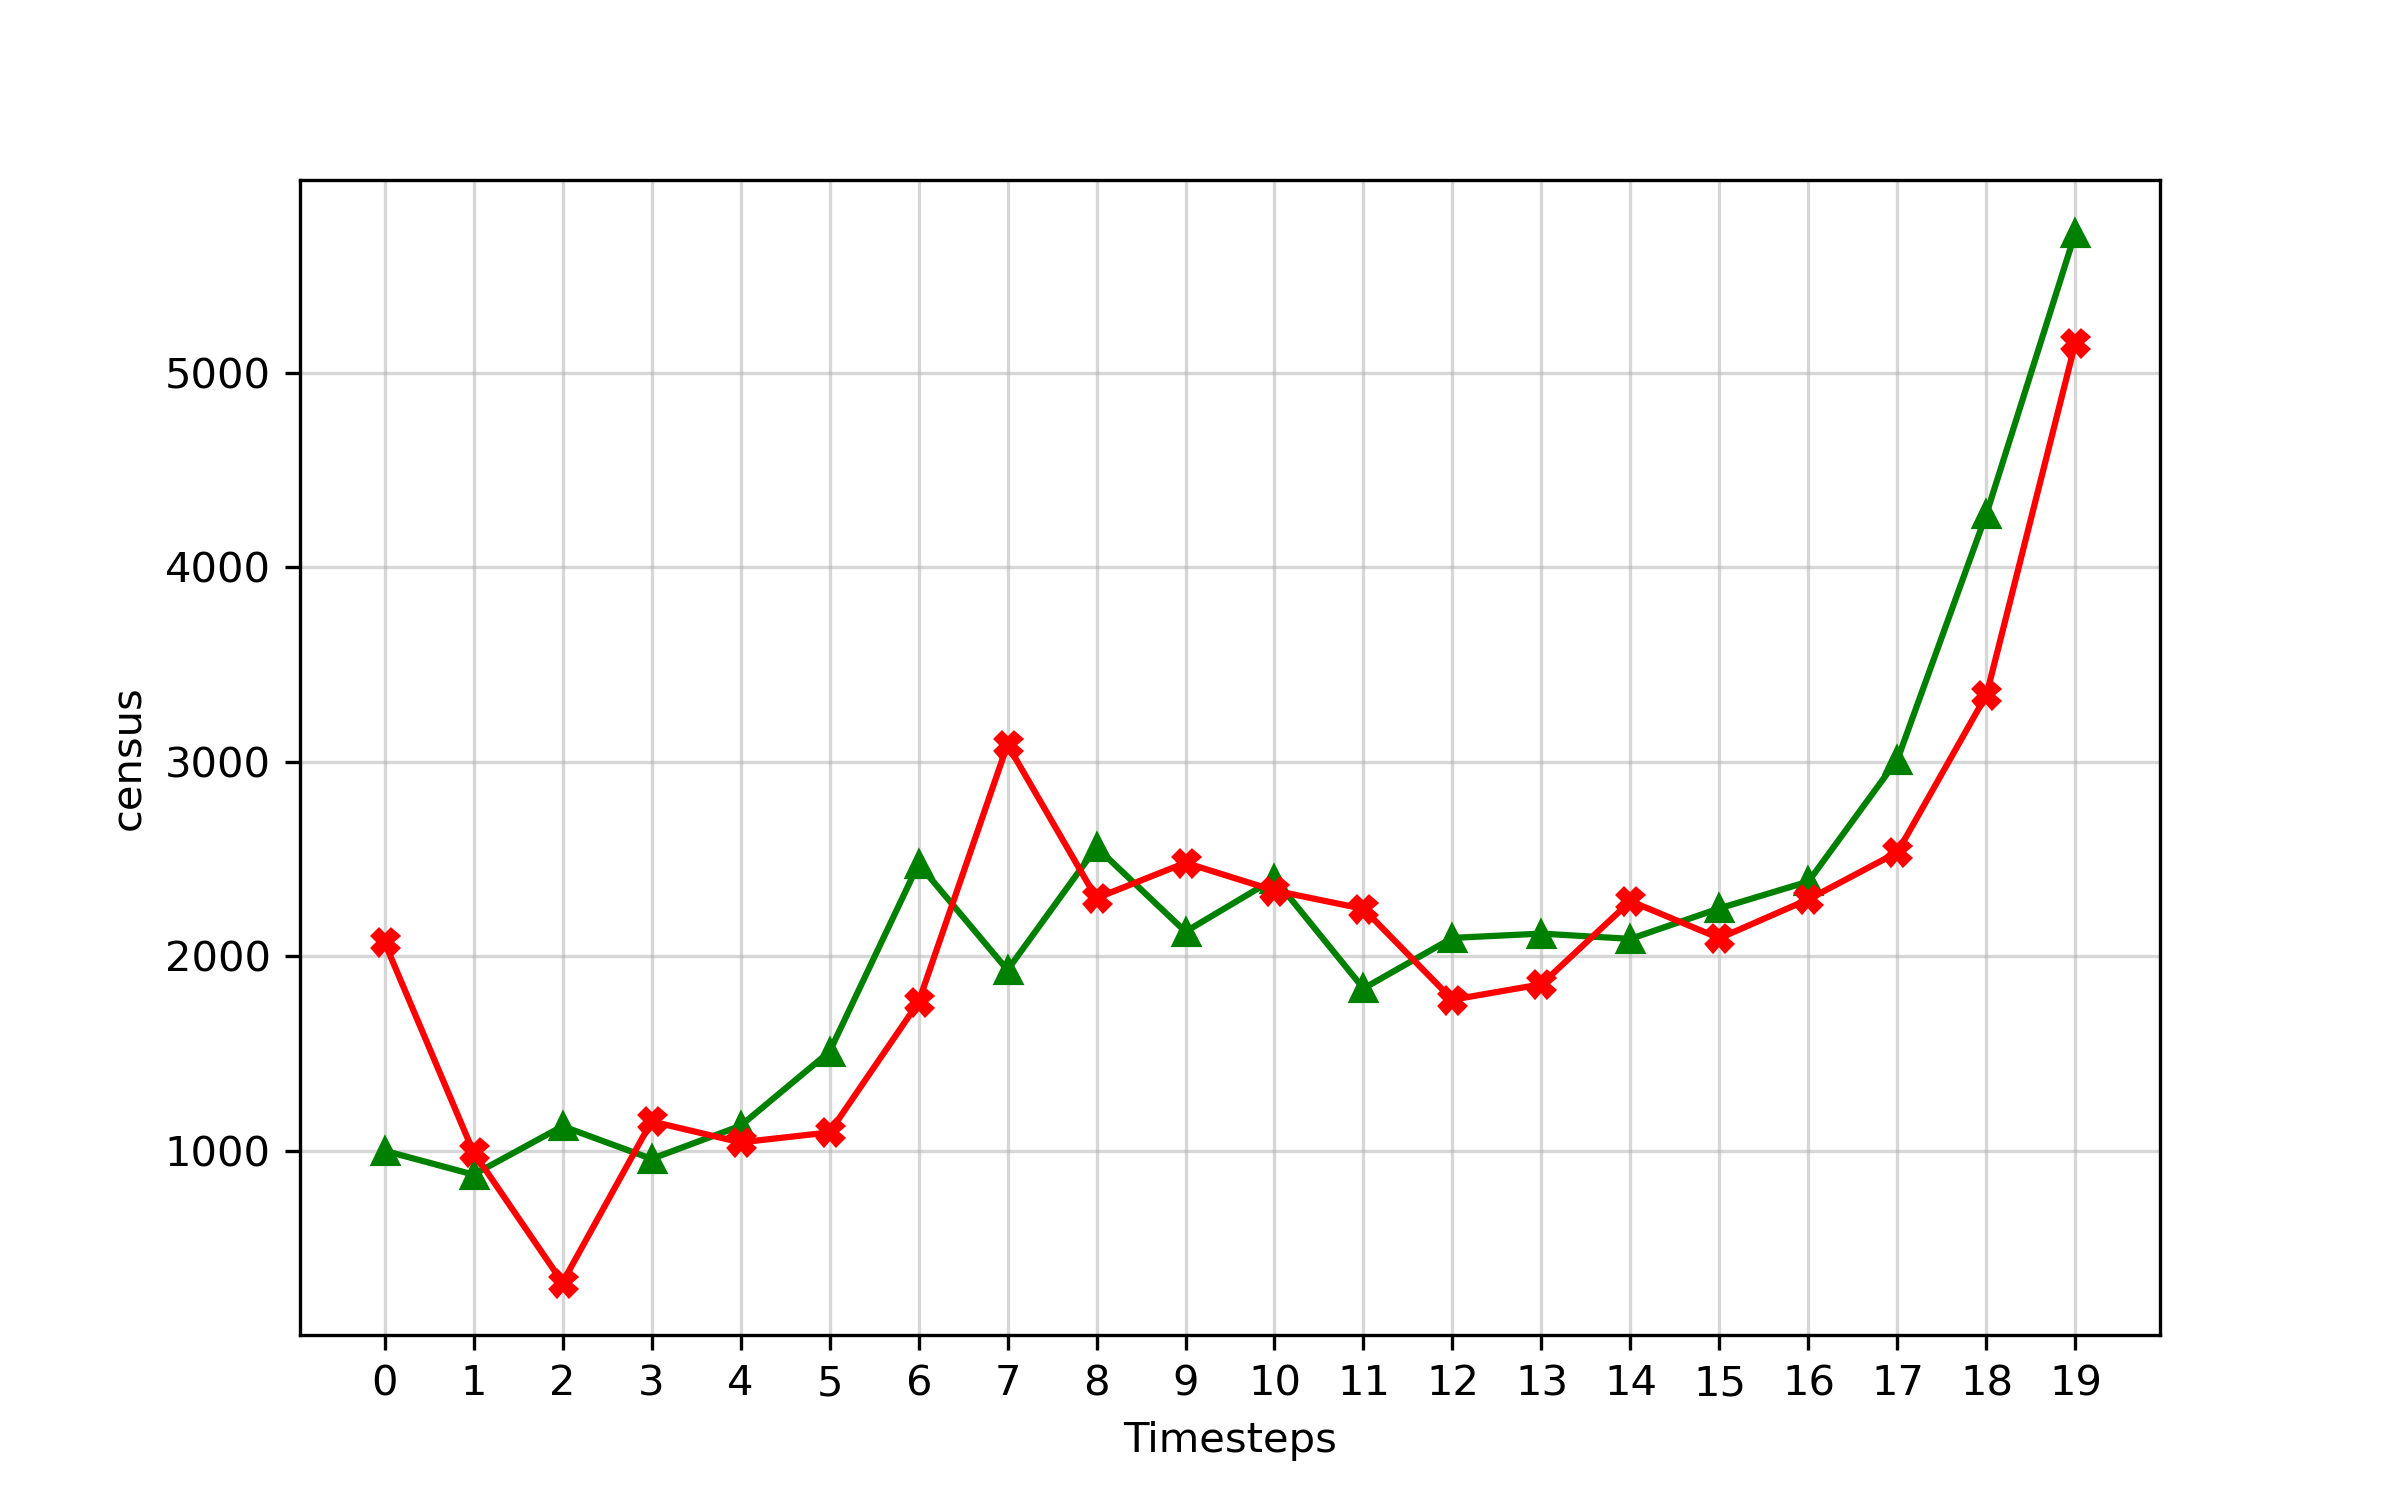
\includegraphics[width=0.7\linewidth]{../private_assets/plot_Census_arima(1,2,0)_predictions_20.png}
% \caption{Gráfico do modelo \textit{\acrshort{arima}}(1, 2, 0), com 20 previsões}
% \end{figure}\par


\begin{figure}[h!]
\begin{floatrow}
\capbtabbox{%
  \begin{tabular}{|c|c|} \hline
    \textbf{"Predict"} & \textbf{"census"} \\ \hline
    2071.4553305007325 & 1000.0 \\ \thinhline
    1486.3564093774662 & 1000.0 \\ \thinhline
    1259.105158633161 & 877.0000000000001 \\ \thinhline
    936.7208987331807 & 1126.0 \\ \thinhline
    891.2391031088812 & 958.0 \\ \thinhline
    664.04646073088 & 1128.0 \\ \thinhline
    1138.8505813208287 & 1509.0 \\ \thinhline
    1536.3068503783759 & 2474.0 \\ \thinhline
    2497.963195964612 & 1928.9999999999998 \\ \thinhline
    2467.5200712884825 & 2560.0 \\ \thinhline
    2953.008515321484 & 2126.0000000000005 \\ \thinhline
    2445.992450723264 & 2398.0 \\ \thinhline
    2346.298572292104 & 1834.0000000000002 \\ \thinhline
    1998.3895774073735 & 2094.0 \\ \thinhline
    1887.2209749046133 & 2116.0000000000005 \\ \thinhline
    2026.4401798934175 & 2089.0 \\ \thinhline
    2003.6514414933647 & 2246.0000000000005 \\ \thinhline
    2335.346340795519 & 2384.0 \\ \thinhline
    2409.007736368172 & 3011.0 \\ \thinhline
    3051.686418045654 & 4274.0 \\ \thinhline
    4442.241881959838 & 5720.0 \\ \hline
  \end{tabular}
}{%
  \caption{Previsões do modelo \textit{\acrshort{arima}}(3, 2, 0), com 20 previsões}%
}
\ffigbox{%
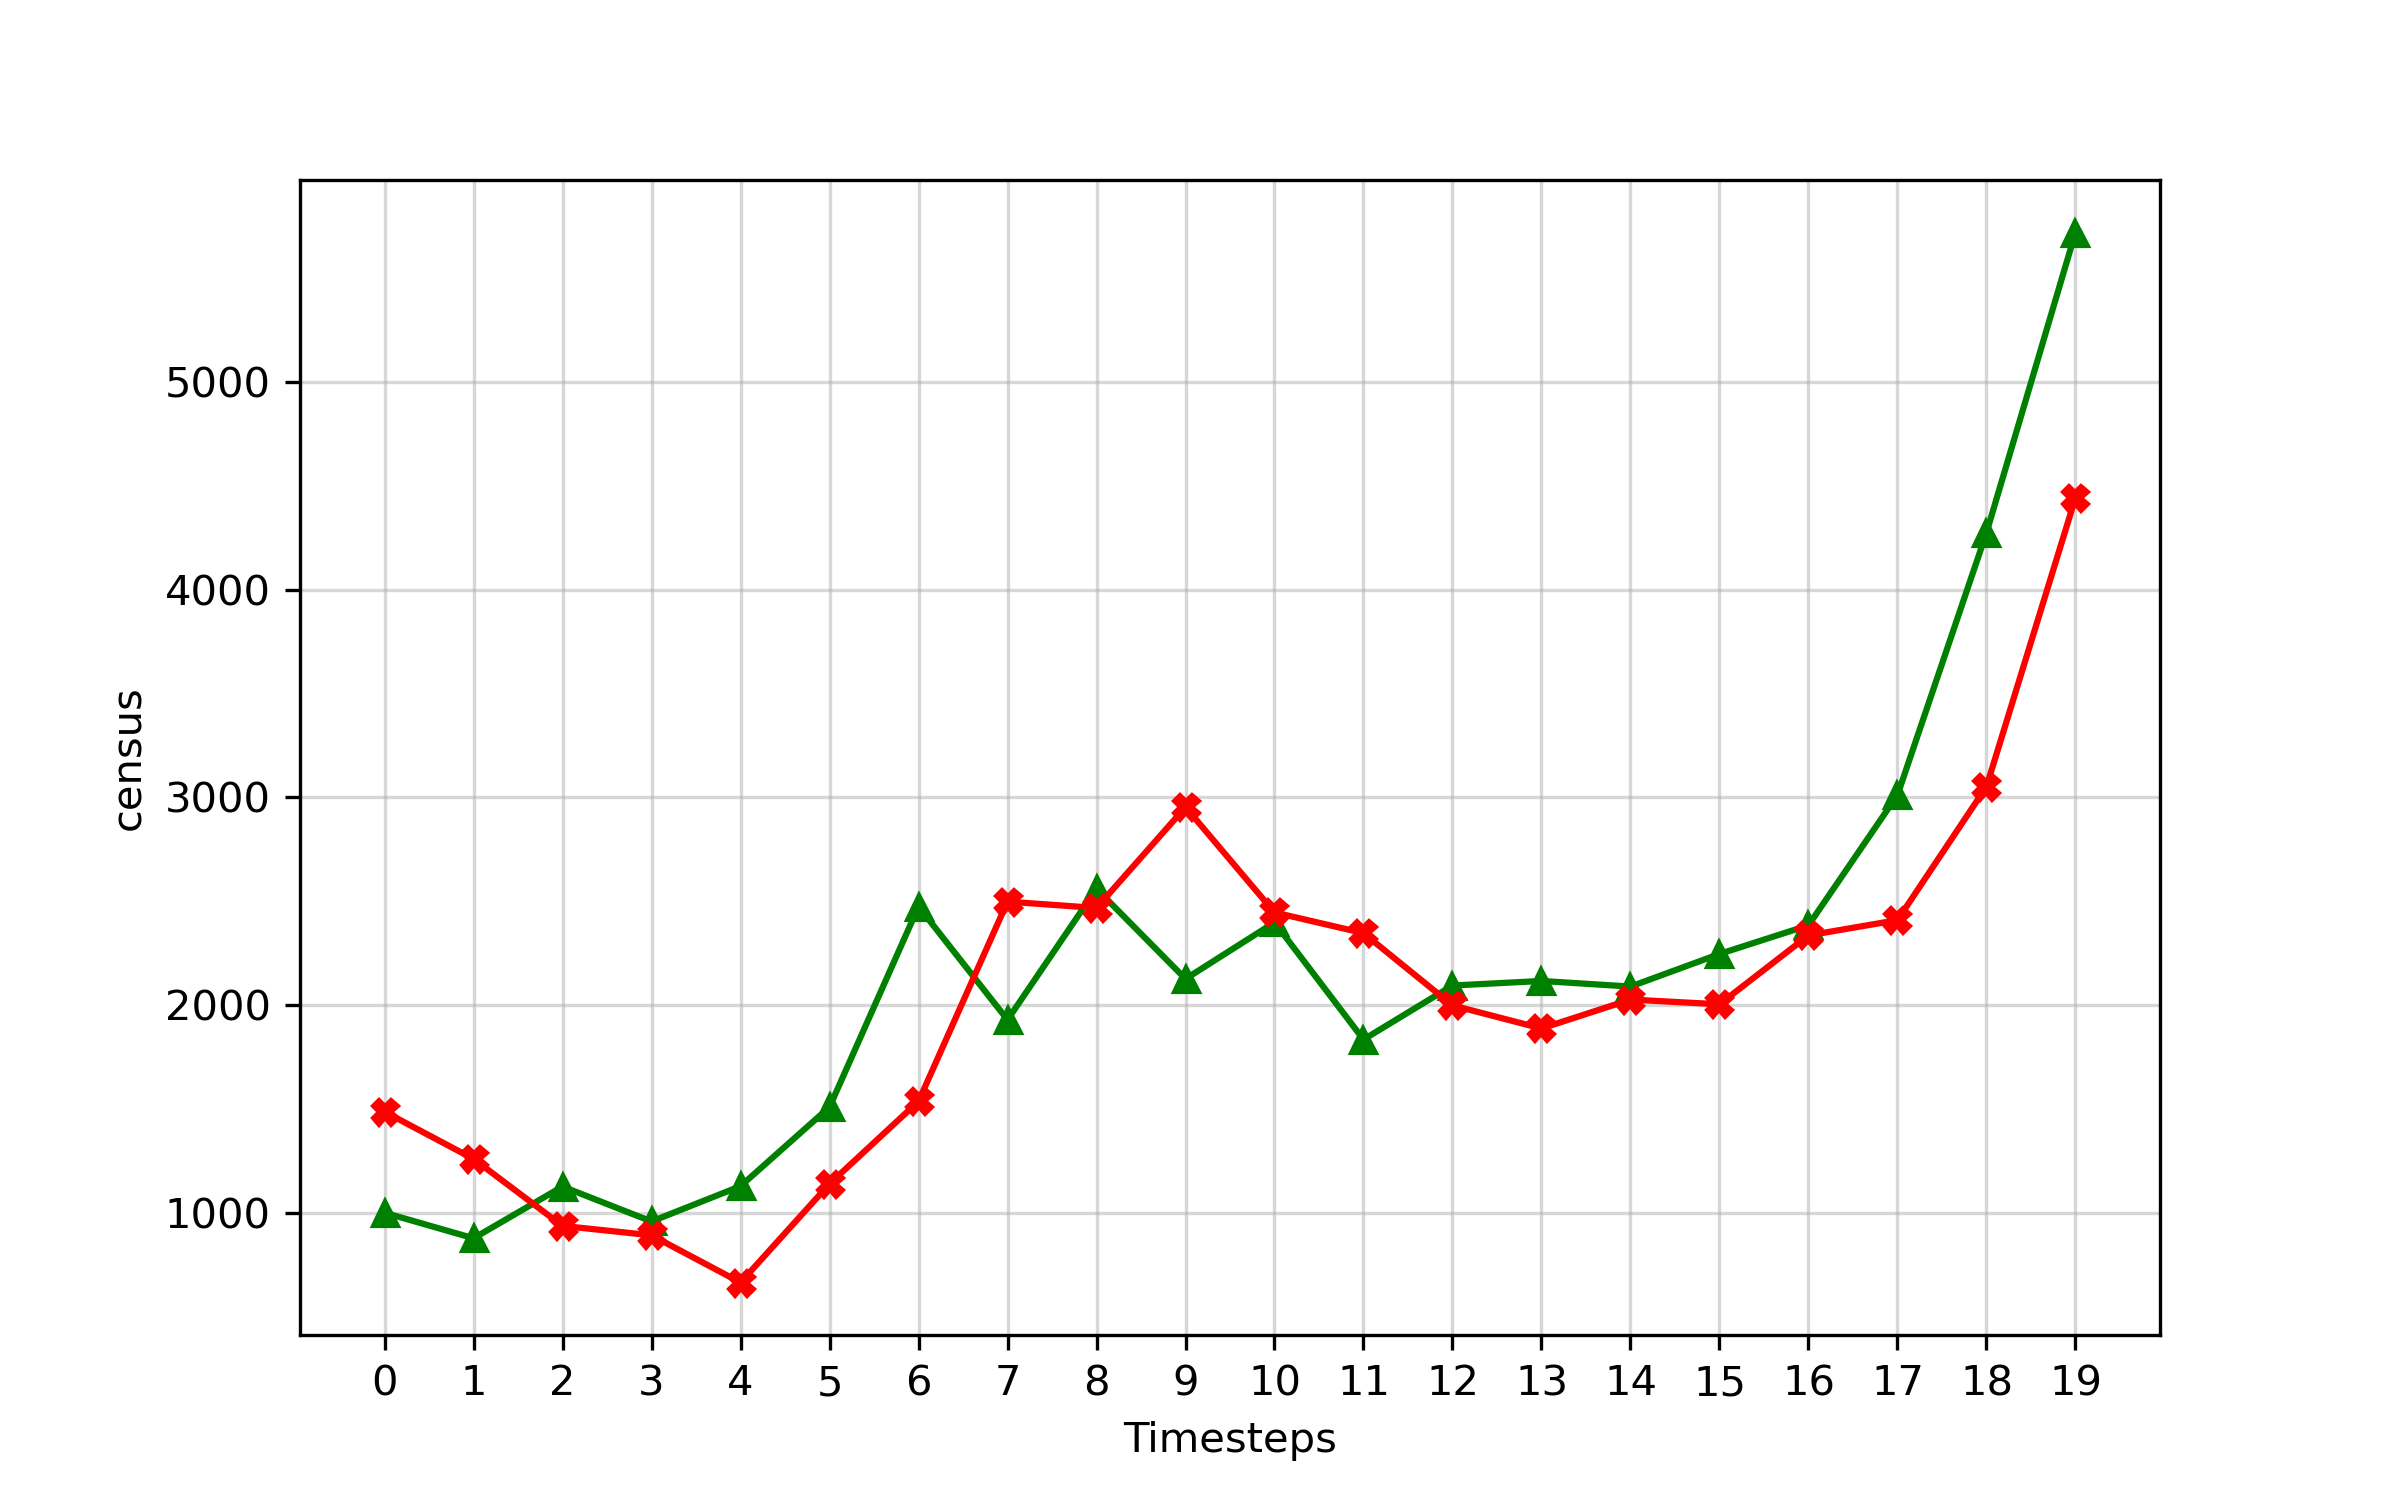
\includegraphics[width=\linewidth]{../private_assets/plot_Census_arima(3,2,0)_predictions_20.png}
}{%
  \caption{Gráfico do modelo \textit{\acrshort{arima}}(3, 2, 0), com 20 previsões}%
}
\end{floatrow}
\end{figure}

\restoregeometry

% \begin{table}[h!]
% \centering
% \setlength{\extrarowheight}{2pt}
% \setlength{\tabcolsep}{10pt}
% \begin{tabular}{|c|c|c|c|c|c|}
% \hline
% \textbf{"Predict"} & \textbf{"speed\_diff"}\\[2pt]
% \hline
% 2071.4553305007325 & 1000.0 \\[2pt]
% \thinhline
% 1486.3564093774662 & 1000.0 \\[2pt]
% \thinhline
% 1259.105158633161 & 877.0000000000001 \\[2pt]
% \thinhline
% 936.7208987331807 & 1126.0 \\[2pt]
% \thinhline
% 891.2391031088812 & 958.0 \\[2pt]
% \thinhline
% 664.04646073088 & 1128.0 \\[2pt]
% \thinhline
% 1138.8505813208287 & 1509.0 \\[2pt]
% \thinhline
% 1536.3068503783759 & 2474.0 \\[2pt]
% \thinhline
% 2497.963195964612 & 1928.9999999999998 \\[2pt]
% \thinhline
% 2467.5200712884825 & 2560.0 \\[2pt]
% \thinhline
% 2953.008515321484 & 2126.0000000000005 \\[2pt]
% \thinhline
% 2445.992450723264 & 2398.0 \\[2pt]
% \thinhline
% 2346.298572292104 & 1834.0000000000002 \\[2pt]
% \thinhline
% 1998.3895774073735 & 2094.0 \\[2pt]
% \thinhline
% 1887.2209749046133 & 2116.0000000000005 \\[2pt]
% \thinhline
% 2026.4401798934175 & 2089.0 \\[2pt]
% \thinhline
% 2003.6514414933647 & 2246.0000000000005 \\[2pt]
% \thinhline
% 2335.346340795519 & 2384.0 \\[2pt]
% \thinhline
% 2409.007736368172 & 3011.0 \\[2pt]
% \thinhline
% 3051.686418045654 & 4274.0 \\[2pt]
% \thinhline
% 4442.241881959838 & 5720.0 \\[2pt]
% \hline
% \end{tabular}
% \caption{Previsões do modelo \textit{\acrshort{arima}}(3, 2, 0), com 20 previsões}
% \end{table}

% \begin{figure}[h!]
% \centering
% 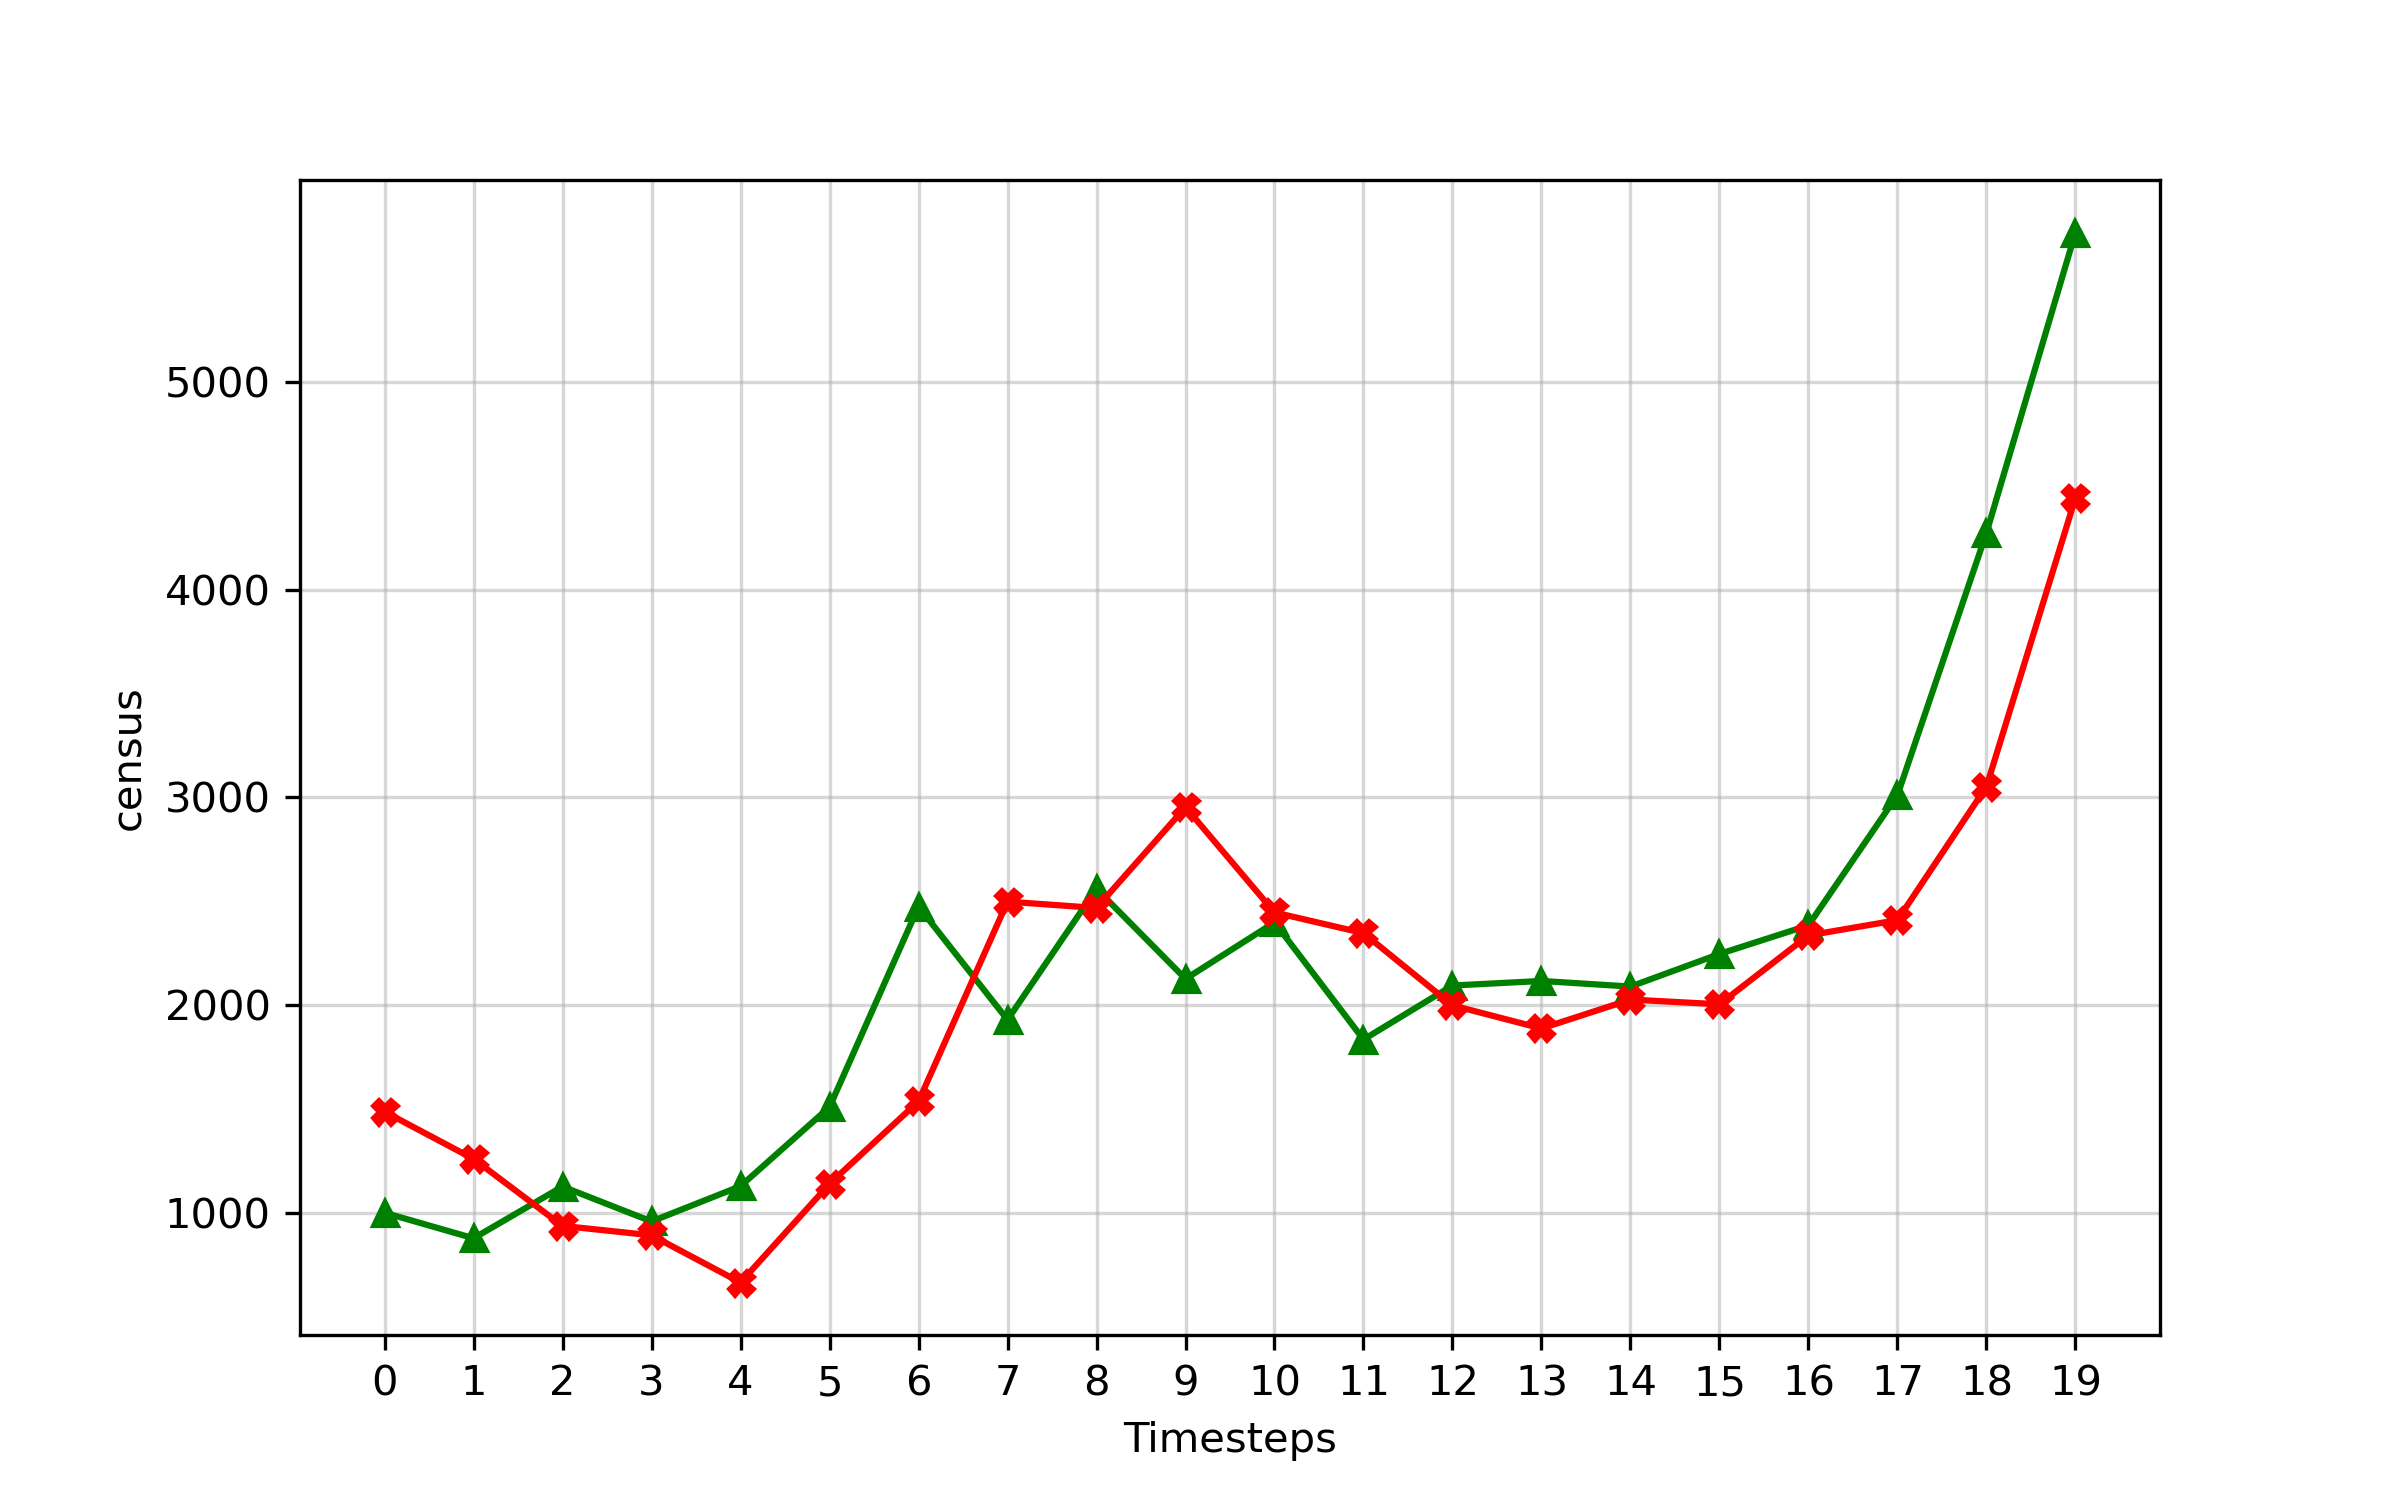
\includegraphics[width=0.7\linewidth]{../private_assets/plot_Census_arima(3,2,0)_predictions_20.png}
% \caption{Gráfico do modelo \textit{\acrshort{arima}}(3, 2, 0), com 20 previsões}
% \end{figure}\par


\newpage

\begin{figure}[h!]
\begin{floatrow}
\capbtabbox{%
  \begin{tabular}{|c|c|} \hline
    \textbf{"Predict"} & \textbf{"census"} \\ \hline
    1938.3248213044278 & 1000.0 \\ \thinhline
    1160.307636030289 & 877.0000000000001 \\ \thinhline
    787.2489987658323 & 1126.0 \\ \thinhline
    686.5435225844557 & 958.0 \\ \thinhline
    984.9846735946015 & 1128.0 \\ \thinhline
    1200.4527870105767 & 1509.0 \\ \thinhline
    1533.760588643199 & 2474.0 \\ \thinhline
    2808.98688952599 & 1928.9999999999998 \\ \thinhline
    2463.9565873495894 & 2560.0 \\ \thinhline
    2876.6031847102568 & 2126.0000000000005 \\ \thinhline
    2075.575964237916 & 2398.0 \\ \thinhline
    2559.965779302652 & 1834.0000000000002 \\ \thinhline
    1678.7683021383232 & 2094.0 \\ \thinhline
    2023.2650400026798 & 2116.0000000000005 \\ \thinhline
    1947.4008439849385 & 2089.0 \\ \thinhline
    2226.007489000049 & 2246.0000000000005 \\ \thinhline
    2262.5125641983063 & 2384.0 \\ \thinhline
    2450.1225894495315 & 3011.0 \\ \thinhline
    3207.1297244942393 & 4274.0 \\ \thinhline
    4722.751309975546 & 5720.0 \\ \hline
  \end{tabular}
}{%
  \caption{Previsões do modelo \textit{\acrshort{arima}}(2, 2, 0), com 20 previsões}%
}
\ffigbox{%
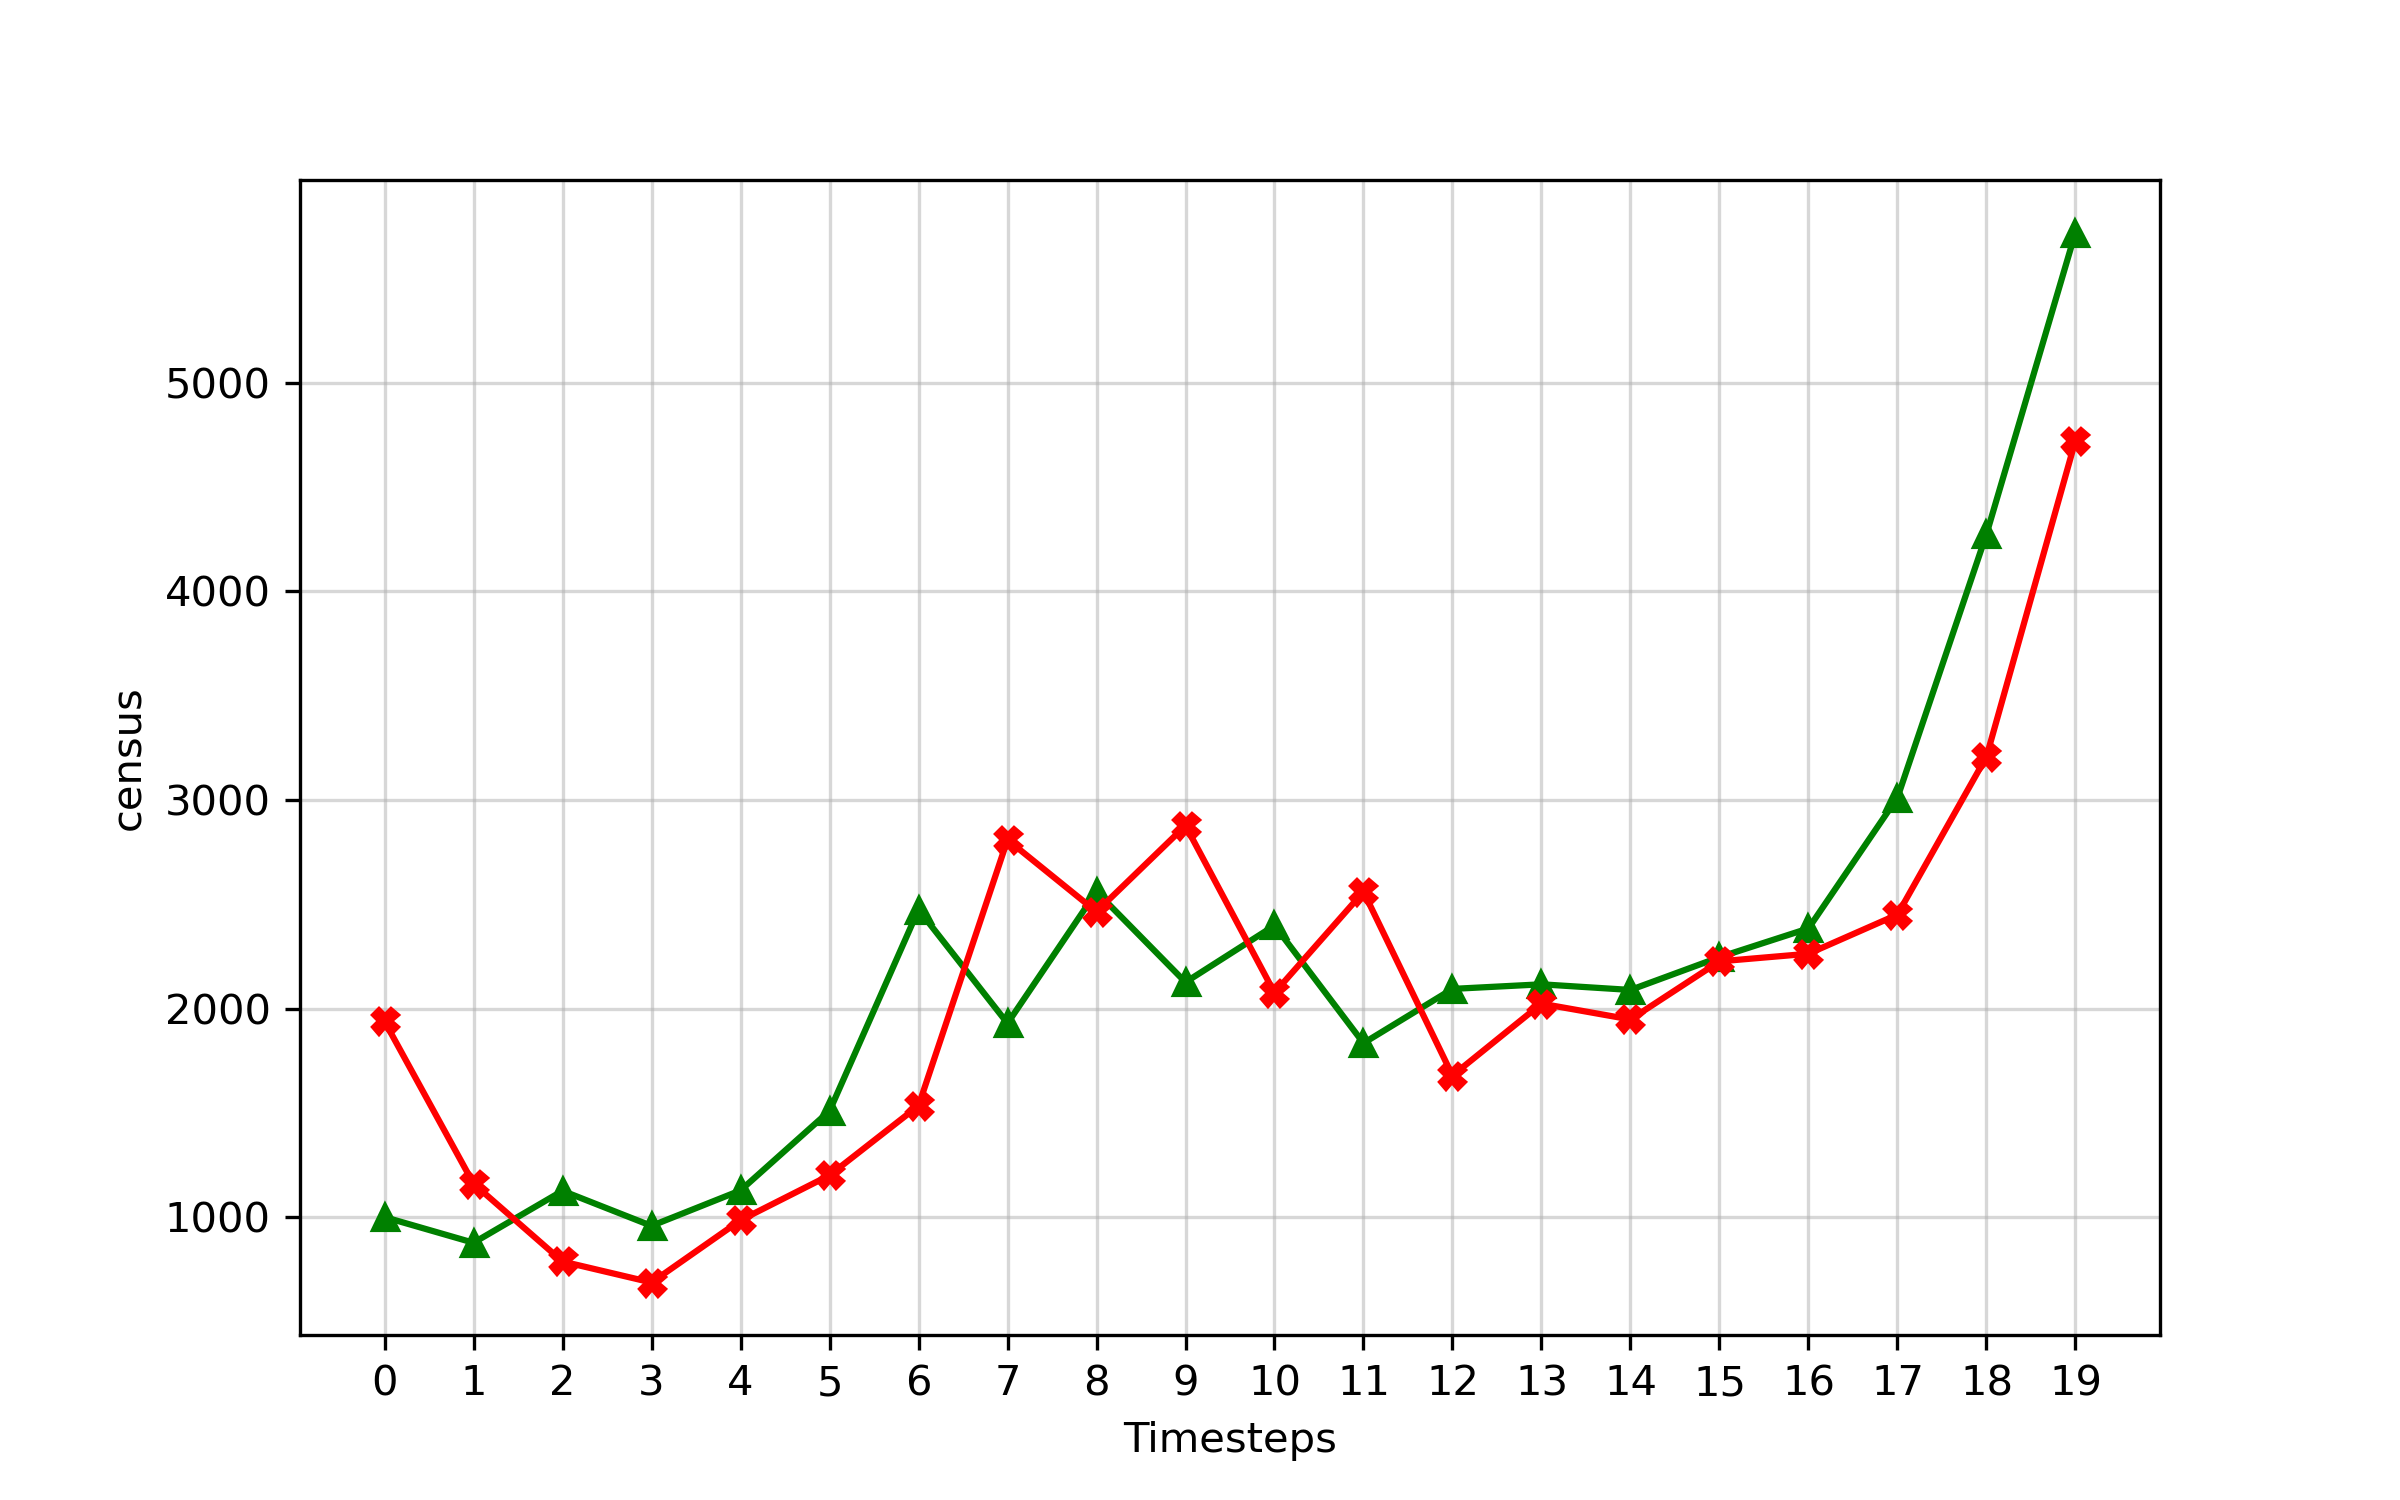
\includegraphics[width=\linewidth]{../private_assets/plot_Census_arima(2,2,0)_predictions_20.png}
}{%
  \caption{Gráfico do modelo \textit{\acrshort{arima}}(2, 2, 0), com 20 previsões}%
}
\end{floatrow}
\end{figure}

% \begin{table}[h!]
% \centering
% \setlength{\extrarowheight}{2pt}
% \setlength{\tabcolsep}{10pt}
% \begin{tabular}{|c|c|c|c|c|c|}
% \hline
% \textbf{"Predict"} & \textbf{"speed\_diff"}\\[2pt]
% \hline
% 1938.3248213044278 & 1000.0 \\[2pt]
% \thinhline
% 1160.307636030289 & 877.0000000000001 \\[2pt]
% \thinhline
% 787.2489987658323 & 1126.0 \\[2pt]
% \thinhline
% 686.5435225844557 & 958.0 \\[2pt]
% \thinhline
% 984.9846735946015 & 1128.0 \\[2pt]
% \thinhline
% 1200.4527870105767 & 1509.0 \\[2pt]
% \thinhline
% 1533.760588643199 & 2474.0 \\[2pt]
% \thinhline
% 2808.98688952599 & 1928.9999999999998 \\[2pt]
% \thinhline
% 2463.9565873495894 & 2560.0 \\[2pt]
% \thinhline
% 2876.6031847102568 & 2126.0000000000005 \\[2pt]
% \thinhline
% 2075.575964237916 & 2398.0 \\[2pt]
% \thinhline
% 2559.965779302652 & 1834.0000000000002 \\[2pt]
% \thinhline
% 1678.7683021383232 & 2094.0 \\[2pt]
% \thinhline
% 2023.2650400026798 & 2116.0000000000005 \\[2pt]
% \thinhline
% 1947.4008439849385 & 2089.0 \\[2pt]
% \thinhline
% 2226.007489000049 & 2246.0000000000005 \\[2pt]
% \thinhline
% 2262.5125641983063 & 2384.0 \\[2pt]
% \thinhline
% 2450.1225894495315 & 3011.0 \\[2pt]
% \thinhline
% 3207.1297244942393 & 4274.0 \\[2pt]
% \thinhline
% 4722.751309975546 & 5720.0 \\[2pt]
% \hline
% \end{tabular}
% \caption{Previsões do modelo \textit{\acrshort{arima}}(2, 2, 0), com 20 previsões}
% \end{table}

% \begin{figure}[h!]
% \centering
% 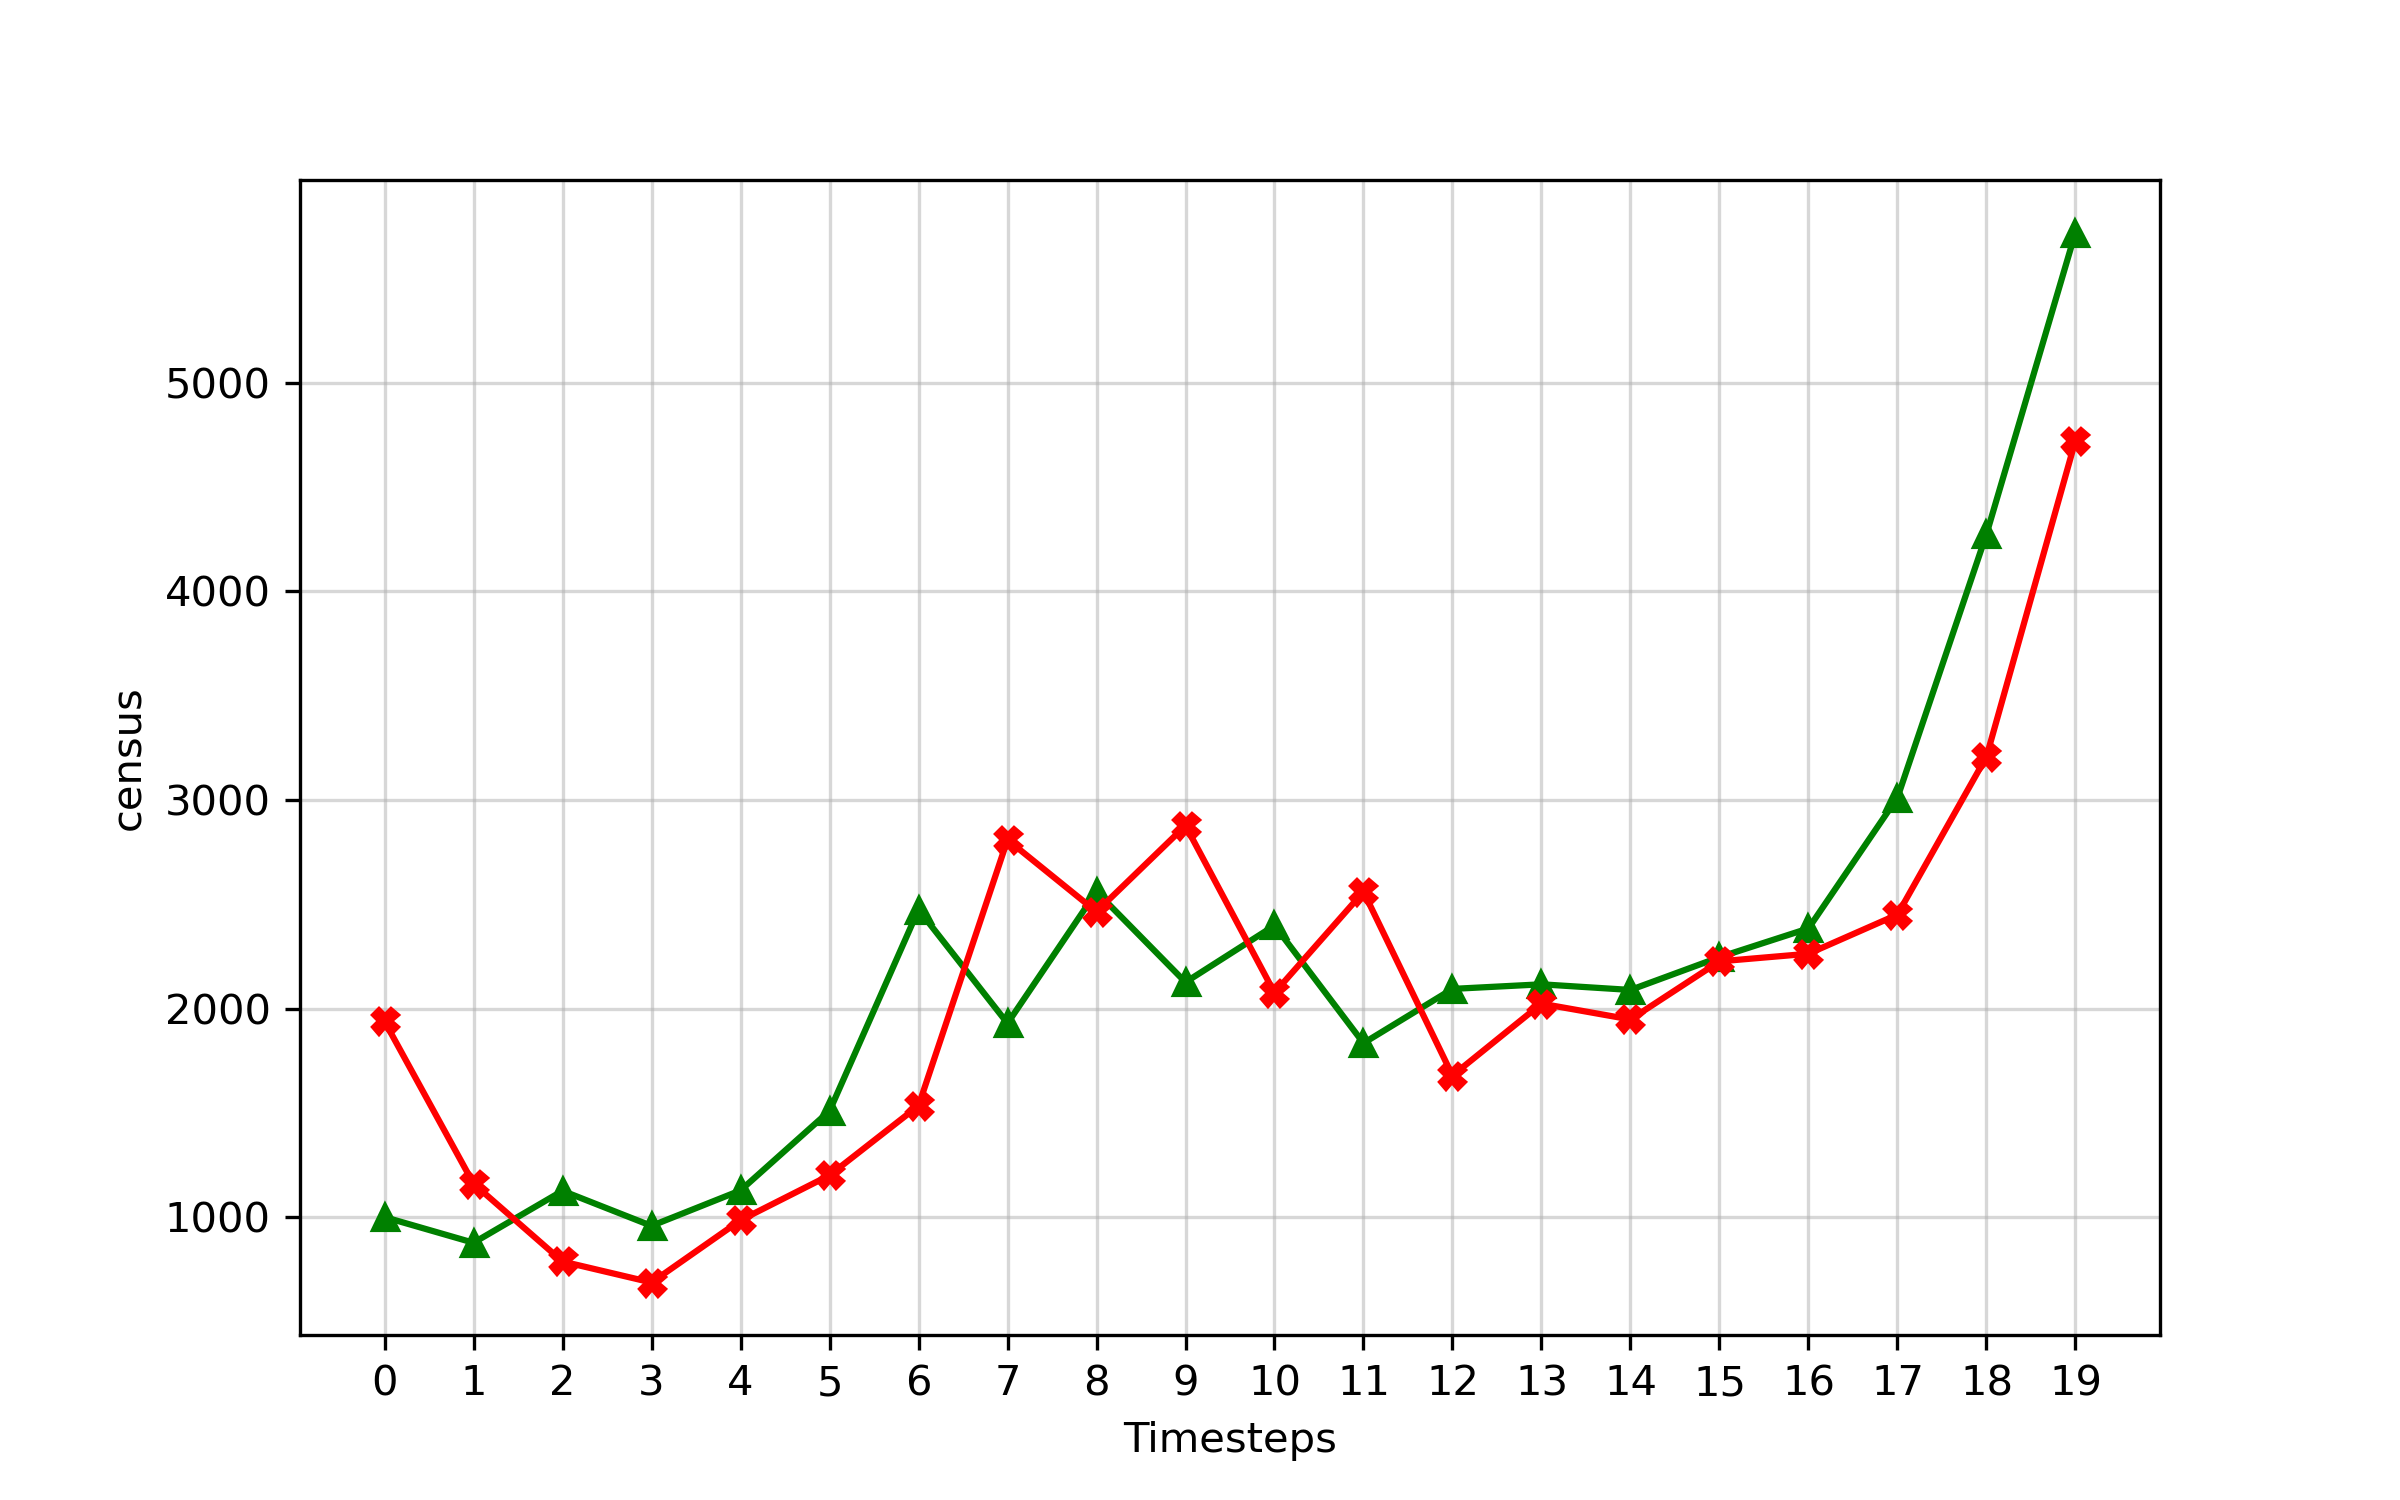
\includegraphics[width=0.7\linewidth]{../private_assets/plot_Census_arima(2,2,0)_predictions_20.png}
% \caption{Gráfico do modelo \textit{\acrshort{arima}}(2, 2, 0), com 20 previsões}
% \end{figure}\par

\vspace{1cm}

Em suma, o modelo mais acertivo foi o modelo representado na tabela 5.8 e na figura 5.6.
Posto isto, podemos concluir que o melhor dia do mês para ir ao quiosque será o dia com
menor população e o pior dia será o dia com maior população. Ou seja, segundo o modelo
da figura 5.4, o melhor dia é o do \textit{timesetp} número 1 e o pior é o \textit{timesetp} número 19. Fazendo a
consulta ao \textit{\gls{dataset}}, podemos concluir que o melhor dia para ir seria no
dia 13 de cada mês e o pior seria no dia 31 (ou 30 para meses com apenas 30 dias).



\newpage
\section{Apresentação dos Impedimentos e/ou Constrangimentos}

Em primeiro, é importante realçar que, na opinião do autor, se um projeto chega ao fim com
sucesso a avaliação geral deve ser positiva. No entanto, podem exister precalços no decorrer
do desenvolvimento do mesmo. Dito isto, os principais pontos em que o autor sentiu mais
dificuldade foram no desenvolvimento do presente documento, bem como no estudo dos modelos
\textit{\acrshort{arima}}, \textit{\acrshort{arimax}}, \textit{\acrshort{sarima}} e
\textit{\acrshort{sarimax}}.\par
Por um lado, o desenvolvimento documento principal foi realizado com a linguagem \textit{LaTeX},
que foi um dos desafios propostos pelo autor ao professor orientador, no entanto, como se
trata da aprendizagem de algo novo, existem sempre mais complicações. Para além disto, o
autor também teve enormes dificuldades em encarar os objetivos do projeto do ponto de
vista teórico.\par
Por outro lado, os algoritmos estudados também provocaram uma certa dificuldade no
desenvolvimento do trabalho. No entanto, como existe uma certa similaridade entre os
modelos, a aprendizagem do primeiro facilitou bastante o entendimento dos restantes.\par
No geral, o trabalho foi positivo, apesar de todos os constrangimentos, visto que foi
concluído com sucesso.

\newpage